\documentclass[12pt]{article}
../../../papers/PJTpreamble.tex
%\usepackage{amsfonts}
\usepackage{setspace}
\linespread{2}
\usepackage{chngcntr}
\usepackage{changebar}
\counterwithin{figure}{section}
\usepackage[top=1in,bottom=1in,left=1.5in,right=1.5in]{geometry}

%\newtheorem{theorem}{Theorem}[section]
%\newtheorem{lemma}[theorem]{Lemma}
\newtheorem{proposition}[theorem]{Proposition}
%\newtheorem{corollary}[theorem]{Corollary}

\newenvironment{proof}[1][Proof]{\begin{trivlist}
\item[\hskip \labelsep {\bfseries #1}]}{\end{trivlist}}
%\newenvironment{definition}[1][Definition]{\begin{trivlist}\item[\hskip \labelsep {\bfseries #1}]}{\end{trivlist}}
\newenvironment{example}[1][Example]{\begin{trivlist}
\item[\hskip \labelsep {\bfseries #1}]}{\end{trivlist}}
%\newenvironment{remark}[1][Remark]{\begin{trivlist}\item[\hskip \labelsep {\bfseries #1}]}{\end{trivlist}}

\newcommand{\qed}{\nobreak \ifvmode \relax \else
      \ifdim\lastskip<1.5em \hskip-\lastskip
      \hskip1.5em plus0em minus0.5em \fi \nobreak
      \vrule height0.75em width0.5em depth0.25em\fi}

% NEED TO INCLUDE:
%Title page
%Committee Approval Sheet                                                                                                                                 %Copyright page (only if copyrighting)
%Dedication page (optional)


\setlength{\headsep}{.5in}

\begin{document}





\pagestyle{empty}
\begin{titlepage}
%The title page must contain the following information:  Title, Name, Degree, Department, University Name, Month and Year of Graduation.  The month of graduation will either be January, May or August.
\begin{center}
INFINITESIMAL PHASE RESPONSE CURVES FOR PIECEWISE SMOOTH DYNAMICAL SYSTEMS\end{center}
\vfill
\begin{center}
by
\end{center}
\begin{center}
Youngmin Park
\end{center}
\vfill
\begin{center}
Submitted in partial fulfillment of the requirements
\end{center}
\begin{center}
For the degree of Masters of Science
\end{center}
\vfill
\begin{center}
Thesis Advisor:  Dr. Peter J. Thomas\\
%With help from MSTP candidate Kendrick Shaw.\\
\end{center}
\vfill
\begin{center}
Department of Mathematics\\ 
\end{center}
\begin{center}
CASE WESTERN RESERVE UNIVERSITY
\end{center}
\vfill
\begin{center}
August, 2013
\vfill
\end{center}
\end{titlepage}

\newpage

% signature page
\begin{center}
\begin{center}
\textbf{CASE WESTERN RESERVE UNIVERSITY}
\end{center}
\begin{center}
\textbf{SCHOOL OF GRADUATE STUDIES}
\end{center}
\vfill
\large


We hereby approve the thesis/dissertation of
\begin{center}\underline{\quad\quad\quad\quad\quad Strunk and White \quad\quad\quad\quad\quad}\end{center}

candidate for the \underline{\quad\quad\quad Master of Science \quad\quad\quad} degree$^*$.
\vfill
\begin{center}\underline{\; Richard Feynman (Committee chair) \;}\end{center}
\begin{center}\underline{\quad\quad\quad\quad\quad Member 2 \quad\quad\quad\quad\quad}\end{center}
\begin{center}\underline{\,\,\quad\quad\quad\quad Member 3 \quad\quad\quad\quad\,\,}\end{center}
\begin{center}\underline{\;\;\;\quad\quad\quad Member 4 \quad\quad\quad\;\;\;}\end{center}

\vfill
\begin{center}(date)\underline{\quad\quad August, 2016 \quad\quad}\end{center}
\vfill

*We also certify that written approval has been obtained for any\\
proprietary material contained therein. 


\end{center}
\normalsize

\newpage

\section*{Dedication}
For my father, Pilho, and sister, Young-Eun.
\newpage

\pagenumbering{roman}
\pagestyle{plain}
\tableofcontents
\newpage

\listoftables
\addcontentsline{toc}{section}{List of Tables}
\newpage

\listoffigures
\addcontentsline{toc}{section}{List of Figures}
\newpage


\section*{List of Abbreviations}
\addcontentsline{toc}{section}{List of Abbreviations}
CPG Central Pattern Generator\\
DI Differential Inclusion\\
iPRC Infinitesimal Phase Response Curve\\
NW Northwest\\
PRC Phase Response Curve\\
PML Piecewise Linear Morris-Lecar\\
PWL Piecewise Linear\\
PWLDS Piecewise Linear Dynamical System\\
$\mathbb{R}$ The Real Numbers\\
$\mathbb{R}^+$ The nonnegative real numbers\\
SW Southwest\\
$||\cdot||$ Arbitrary Norm\\
\newpage

\section*{Acknowledgements}
\addcontentsline{toc}{section}{Acknowledgements}
Special thanks to Dr.~Thomas, Dr.~Chiel, and Kendrick Shaw for their unwavering guidance and support.  
\newpage



%\section{List of Abbreviations}
%\section{Glossary}
%\doublespace

\section*{Abstract}
Dynamical systems with discontinuous right-hand sides are utilized to great effect in mathematical biology (Coombes 2008, Glass and Kauffman 1973, McKean 1970), including models of central pattern generators (CPGs) involved in motor control (Spardy et al. 2011, Shaw et al. 2012).  CPG models typically exhibit limit cycle dynamics; the infinitesimal phase response curve (iPRC) quantifies sensitivity of such models to external inputs (Ermentrout and Terman 2010).  Piecewise smooth dynamical systems may have discontinuous iPRCs.  In this thesis, we formulate the boundary conditions necessary for obtaining the iPRC for general piecewise smooth dynamical systems by solving an adjoint equation, thereby improving upon two known methods used to solve for the iPRC in the context of piecewise linear dynamical systems.
\newpage



\pagestyle{headings}
\pagenumbering{arabic}
\section{Introduction}

%\subsection{Background}
%\begin{itemize}
 %\item Possible starting points:
 %\begin{itemize}
%  \item How action potentials work:\\
%  Draft
%  \item dreivation of hh-like dyn. systems (this might be useful for setting the context)
%  \item benefits of neurobiological experiments on aplysia. Chiel lab first to look at mechanics of feeding
% \end{itemize}
% \cite{Coombes:2008:SIADS,Gebert20071148,Glass1973103,ShawParkChielThomas2012SIADS,SpardyEtAlRubin2011a,SpardyEtAlRubin2011b}
 Central pattern generators (CPGs) are networks of neurons that produce rhythmic outputs even in the absence of sensory feedback.  Some rhythmic processes controlled by CPGs include breathing (by the pre-B\"{o}tzinger complex in mammals \cite{Butera+Rinzel+Smith:1999a:JNPhys,Butera+Rinzel+Smith:1999b:JNPhys}), locomotion \cite{CohenErmentroutKiemelKopellSigvardtWilliams:1992:TrendsNsci,SpardyEtAlRubin2011a,SpardyEtAlRubin2011b}, and mastication \cite{LundKolta:2006}.  CPGs may be modeled using limit cycles, with the CPG circuit embedded inside biomechanical systems.  These systems are often subject to environmental variability, which may include loads and mechanical resistance.  In many circumstances, it would be disadvantageous if the motion produced by the CPG did not take into account these external forces.  For a simple example of how CPGs robustly adapt to forces, imagine chewing hard bubble gum.  Stiff gum requires extra force to soften, leading to an increase in the duration of a chewing cycle \cite{Plesh1986}.  
 In general, an animal may need to apply a force for longer or shorter times, which could be accomplished by lengthening or shortening the time spent in a portion of a CPG limit cycle.  %One possible mathematical description for this kind of control involves applying small perturbations to a limit cycle passing near fixed points.
 
%Environmental variability is reflected in variations in repetitive patterns.  Observations by the Chiel lab of spontaneous activity in motor neurons of the sea slug \textit{Aplysia californica} involved in feeding behavior exhibit significant variability in the timing of feeding motions, both \textit{in vitro} and \textit{in vivo}.  Understanding CPG timing in the experimentally tractable \textit{Aplysia} system may help in understanding CPG timing in general.
 
%In order to model such variable cycles, we use neuromechanical models in the form of differential inclusions (DIs) \cite{Filipov1988} that allow for arbitrarily long forces.%.  These models may involve using differential inclusions (piecewise linear dynamical systems) which have limit cycles with close passage to fixed points.  %  Understanding how the timing of a CPG responds to external perturbations -- from patterned inputs from the brain to 
%external mechanical resistance -- is central to the biological motivation behind this thesis.
 
%In order to understand how central pattern generators (CPGs) respond to perturbations, we use the buccal mass of the mollusk \textit{Aplysia Californica}.  There are two advantages to performing neurobiological studies on this animal: first, it is possible to distinguish the different states of its feeding mechanism, and the neurons and nerves controlling the many muscles of the buccal mass have been characterized \cite{ }.  Second, the buccal mass remains physiologically active for long times after removal from the animal, allowing for relatively tractable neurobiological experiments \textit{in vitro} (and indeed \textit{in vivo}). In the living animal, perturbations to the feeding CPG tend to happen during feeding.  The food, typically seaweed, may change texture along its length, or the slug may bite down on inedible material.  In either case, the CPG adaptively responds by adjusting the frequency and power behind each bite.

%We are interested in understanding the underlying dynamical system that  allows for robust responses of the feeding CPG.  We can discretize the feeding mechanism into three distinct states: protraction, grasping, and retraction.  With an appropriate metric, we can quantify exactly where the feeding mechanism is with respect to these three states and plot them in state space (Fig.~\ref{fig:aplysia-state-space}).In addition to experimentally finding the phase response properties of the feeding CPG,
 %as an explanation for the spontaneous variability of the timing,
 
 %, and as a mechanism to describe the way in which animals lengthen the time spent in one portion of the CPG limit cycle
 In \cite{ShawParkChielThomas2012SIADS}, Shaw et al. hypothesized that the relative timing of different components of feeding motions could be controlled by manipulating the proximity of trajectories to equilibrium points.  We are interested in this possibility as a mechanism for controlling timing.  Experimental observations suggest the underlying dynamics of the CPG could consist of a limit cycle passing closer to or farther from one or more fixed points.  External or internal perturbations that shift near-limit cycle trajectories closer or father from fixed points could thereby slow down or speed up these trajectories, providing a mechanism for significantly changing the duration of a particular phase of a CPG cycle.
 
   Infinitesimal phase response curves (iPRCs) quantify changes in timing of an oscillator in response to perturbations. iPRCs arise from the reduction of an oscillator to a single phase variable, which we will discuss further below.  In \cite{ShawParkChielThomas2012SIADS}, Shaw et al. analyzed a one-parameter family of planar differential equations with limit cycles whose proximity to fixed points varied parametrically.  They discovered anomalous structure in the shape of the iPRC and the sensitivity of the underlying limit cycle.  In order to carry out a more complete analysis of the shape of the iPRC, Shaw et al. constructed a related family of piecewise linear (PWL) planar differential equations (the iris system, defined in Appendix \ref{app:iris}).  The analytical tractability of this system led to the exact derivation of an iPRC, which provided insight into the 
behavior of the smooth nonlinear system.
   
   Differential equations where the right hand side is piecewise continuous, on a collection of domains partitioning the phase space, is a generalization of smooth differential equations, and are referred to as differential inclusions (DIs) \cite{Filipov1988}.  DIs, discussed further in Section \ref{sec:iprcs_and_dis}, appear in a variety of contexts including control theory \cite{PadenSastry:1987}, as well as in mathematical biology for modeling rhythmic processes.  For example, the switch between swing and stance in models of bipedal animals or quadrupeds is represented by defining two sets of differential equations, and switching the dynamics by a threshold condition \cite{SpardyEtAlRubin2011a,SpardyEtAlRubin2011b}.  In addition, piecewise linear DIs have proved useful as approximations to biological dynamics modeled by smooth systems.  In the study of gene regulatory networks, piecewise linear dynamical systems (PWLDS) play an important role in modeling gene regulatory networks (Glass networks) \cite{
Glass1973103}. In some networks, genes switch almost instantaneously and 
determine a new set of rules for protein production.  This rapid switch is assumed to be instantaneous, and the protein production dynamics are assumed to be linear, leading to a system of piecewise linear (PWL) differential equations \cite{Gebert20071148}.  In the study of gap junction coupled neural networks, PWL approximations to smooth systems allow for analytical solutions which would not be available in the corresponding smooth system \cite{Coombes:2008:SIADS}.  In order to study the limit cycles approaching a sequence of saddle equilibria, we will consider PWL systems where each domain contains a saddle point with the dynamics determined by the linearization about the corresponding saddle of the smooth system.


% MOVE THIS TO DISCUSSION: in this thesis we considered LCs passingn near a succession of fixed points.  this construction was motivated by afraimovich et al. on stable heteroclinic cycles.  Whereas can use limit cycles to model CPGs \cite{Ijspeert:2008:NeuralNet}, we are interested in models with arbitrarily long cycles, therefore it is natural to consider limit cycles passing near saddle points of a heteroclinic cycle \cite{AfraimovichTristanHuertaRabinovich:2008:Chaos}.

% The time it takes it gets through the cycle is dominated by time spent near each fixed point. If one linearizes the flow near the fixed point, it is natural to consider a series of linearized dynamics, one for each fixed point that the limit cycle approaches.  
%It is natural to approximate the nonlinear dynamics with a PWL system for which each domain obeys the linear dynamics associated with one of the saddle points comprising the heteroclinic cycle.
   
   
For limit cycles in general nonlinear systems of differential equations, an explicit expression for the iPRC is known in only a few cases \cite{BrownMoehlisHolmes:2004:NeComp}. In most cases, the iPRC must be obtained through an approximation, typically by numerical integration of an adjoint equation (Section \ref{sec:prc_and_adjoint} and Appendix \ref{app:adjoint_eq}).  Shaw et al. used a direct approach by combining the effects of perturbations on timing and position of trajectories, deriving an exact iPRC with discontinuous jumps at some boundaries and not at others \cite{ShawParkChielThomas2012SIADS}.  Coombes studied two piecewise linear models that have continuous iPRCs and formulated a derivation for the iPRC that applies naturally to both models (and indeed similar classes of FitzHugh-Nagumo-type models) \cite{Coombes:2008:SIADS}.  However, the approach in \cite{Coombes:2008:SIADS} does not take into account possible discontinuities in the iPRC (such as those in the iris system, Appendix \ref{app:iris_summary} and \ref{app:iris}).  In 
this thesis, we provide a concise, closed-form analytic expression for the discontinuity of the iPRC at the domain boundary of any planar piecewise linear differential equation, as well as for more general DIs including nonlinear piecewise smooth differential equations, satisfying a natural boundary condition.  This expression, combined with a solution to the adjoint equation (solvable in closed form for piecewise linear domains), provides a complete picture of the iPRC for a broad class of planar piecewise smooth differential equations.



%Read up on the PRC/iPRC related to weakly coupled oscillators!

% what else? (but what roles does the iPRC play in glass networks? On a conceptual level it could tell us about the effects of chemically perturbing concentrations)

% \begin{itemize}
%  
%  \item Interplay between proprioceptive input, noise, and CPG.
%  \item Biological evidence and justification for sine system model
% \end{itemize}


%\subsection{Motivation}
 %What about biological motivation?\\

 %Implications of understanding iPRC in terms of arc length:\\
 
\subsection{Phase Response Curves and the Adjoint Equation}\label{sec:prc_and_adjoint}
The phase response curve (PRC) is a periodic function quantifying the change in timing of a limit cycle in response to  instantaneous perturbations of a trajectory.  Perturbations may include mechanical feedback, proprioceptive feedback, or input from neighboring oscillators.  Here, we focus on mechanical and proprioceptive feedback.  The techniques of linear perturbation theory dictate the use of small perturbations.  Moreover, in the study of near-homoclinic or near-heteroclinic systems, basins of attraction are often small. In the limit of small perturbations, one obtains the infinitesimal phase response curve (iPRC).

The iPRC is typically defined in the context of smooth systems \cite{ErmentroutTerman2010book}.  Here, we explore the validity of the iPRC and related tools in the context of piecewise smooth and piecewise linear dynamical systems.  For the convenience of the reader, we review the classical terms needed to define the iPRC and the adjoint equation that it satisfies.  Then we examine how these notions extend to limit cycles arising from piecewise smooth dynamics.

Consider a deterministic system of autonomous ordinary differential equations in $\mathbb{R}^n$ with smooth right-hand side:
  \begin{equation}
  \frac{dx}{dt} = F(x),
  \end{equation}
where $F : \mathbb{R}^n \rightarrow \mathbb{R}^n$ is a $C^\infty$ map.
\begin{definition}
 A non-constant solution $x(t)$ (with initial condition $x(0) = x_0$) is called \underline{periodic} with period $T$ if there exists a real constant $T$ such that 
\begin{equation}
 x(t) = x(t+T), \quad \forall t \in \mathbb{R}^+,
\end{equation}
where $T > 0$ is the least such number.
\end{definition}

\begin{definition}
 A $T$-periodic stable limit cycle, $\gamma$, is an isolated $T$-periodic solution with the property that nearby solutions converge to the set $\Gamma = \{\gamma(s): \quad s \in [0,T)\}$ as $t \rightarrow \infty$.
\end{definition}
  We will denote the set of initial conditions for which trajectories converge to $\Gamma$ as the basin of attraction (B.A.).

  \begin{definition} The \underline{phase} of a limit cycle with period $T$ is a function $\theta: \gamma \rightarrow S^1 = [0,1)$ such that
  \begin{equation}
  \frac{d}{dt}\left (\theta(\gamma(t)) \right ) = 1/T,
  \end{equation}
  where $\theta = 0$ is chosen arbitrarily.
  \end{definition}
  Fig.~\ref{fig:dthetadt} illustrates the relationship between a conductance-based model and the corresponding phase variable.
  
  \begin{figure}[h!]
   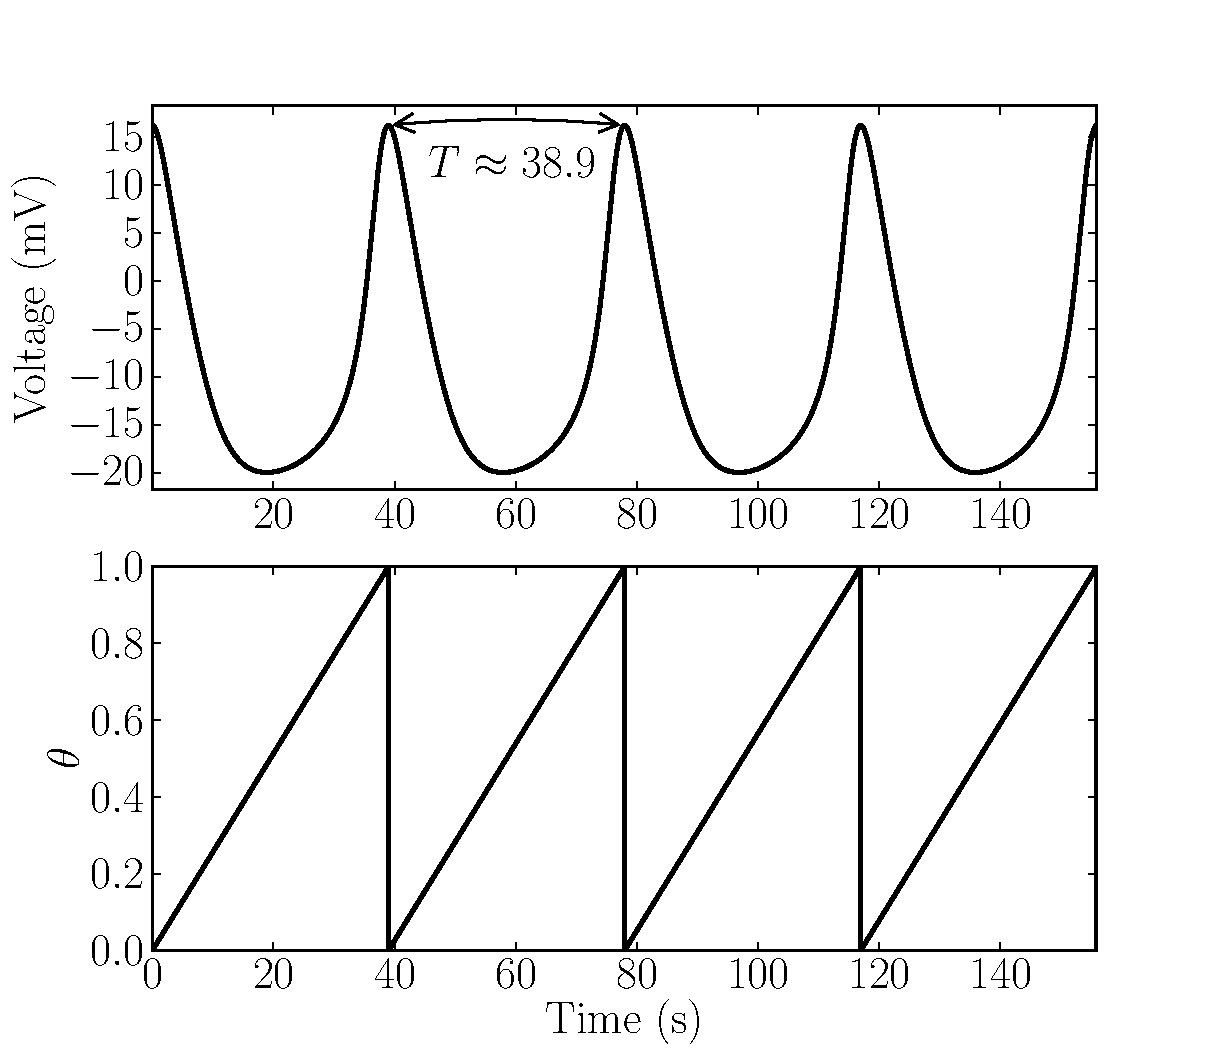
\includegraphics[width=\textwidth]{dthetadt_fig.pdf}
   \caption[The phase function $\theta$ over time]{The phase function $\theta$ over time.  The top panel is a voltage trace of a limit cycle of the Morris-Lecar model (defined in Appendix~\ref{app:morris-lecar}).  The bottom panel shows the corresponding phase values with respect to the limit cycle.  Here, we have defined zero phase corresponding to peak voltage, as is typical with many neurobiological models.}
  \label{fig:dthetadt}\end{figure}
  If the limit cycle is hyperbolic\footnote{A hyperbolic limit cycle is such that the modulus of the Floquet multipliers corresponding to the eigenvectors transverse to the limit cycle are strictly less than unity \cite{Guckenheimer1975JMathBiol}.}, then given a point $x_0 \in B.A.$, there exists a unique $\theta(x_0)$  such that 
  \begin{equation}\label{eq:thetax0}
    \lim_{t \rightarrow \infty} || x(t) - \gamma(t + T\theta(x_0)) || \rightarrow 0.
  \end{equation}
  \begin{definition}
  The value $\theta(x_0)$ in Eq.~\eqref{eq:thetax0} is the \underline{asymptotic phase} of the point $x_0$.
  \end{definition}
  By construction, the asymptotic phase function, $\theta(x)$, has the property that
  \begin{equation}
   \frac{d }{dt}\left (\theta(x(t)) \right ) = 1/T,
  \end{equation}
  for any trajectory in B.A.
  
  
  \begin{definition}
  An \underline{isochron} is a level curve consisting of points that share the same asymptotic phase (Fig.~\ref{fig:sample-phase}).  In other words, two points $x_0,x_1 \in B.A.$ are on the same isochron if for two trajectories $\hat{x}_1$ and $\hat{x}_2$,
  \begin{equation}
   \lim_{t \rightarrow \infty} |\hat{x}_1(t) - \hat{x}_2(t)| = 0,
  \end{equation}
  where the trajectories have initial conditions, $\hat{x}_1(0) = x_0$ and $\hat{x}_2(0) = x_1$.
  \label{def:isochron}
  \end{definition}

\begin{figure}
\begin{center}
 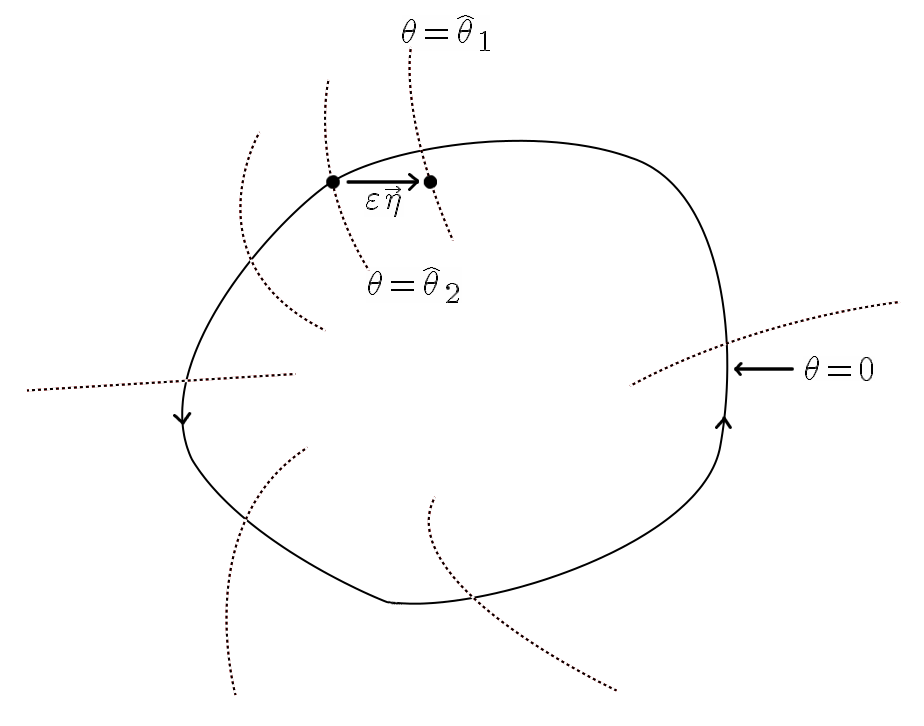
\includegraphics[width=.75\textwidth]{isochron-demo.png}
\end{center}
 \caption[Isochrons of a planar limit cycle]{Isochrons of a planar limit cycle.  Dashed lines represent isochrons, which are level curves of points sharing the same asymptotic phase.  In this example, a small perturbation of size $\varepsilon$ in direction $\eta$ at phase $\hat{\theta}_2$ pushes a trajectory to a different isochron, leading to a phase shift of $\Delta\theta = \hat{\theta}_1 - \hat{\theta}_2$.}
\label{fig:sample-phase}\end{figure}

The change in phase, $\Delta \theta$, in response to a perturbation of size $\varepsilon$ in the unit vector direction $\eta$, depends on the time at which the perturbation occurs.  To derive the infinitesimal phase response curve, provided the asymptotic phase function $\theta$ is $C^1$, we expand the function to first order in $\varepsilon$.
\begin{equation}\label{eq:iprc_derivation}
\begin{split}
 \theta(\gamma(t) + \varepsilon \eta) &= \theta(\gamma(t)) + \varepsilon D\theta(\gamma(t))\cdot \eta + O(\varepsilon^2),\\
\Delta \theta &= \theta(\gamma(t) + \varepsilon \eta) - \theta(\gamma(t)) = \varepsilon D\theta(\gamma(t))\cdot \eta + O(\varepsilon^2),\\
\lim_{\varepsilon \rightarrow 0} \frac{\Delta \theta}{\varepsilon} &= D\theta(\gamma(t))\cdot \eta =: z(t) \cdot \eta.
\end{split}
\end{equation}
We define the gradient of the phase function, $D\theta(\gamma(t))$, to be the iPRC, $z(t)$.  Explicit solutions exist for only a few cases (see Appendix \ref{app:explicit_iprcs}).  The iPRC may be approximated by direct perturbations, or alternatively by solving an adjoint equation,
\begin{equation}
 \frac{dz}{dt} = A(t) z(t),
\label{eq:adjoint}\end{equation}
where $A(t) = -DF^T(\gamma(t))$, the negative transpose of the linearization of the vector field $F$ evaluated along the limit cycle $\gamma$.  See Appendix \ref{app:adjoint_eq} for a derivation of the equation.

%      \begin{figure}[h!]
%  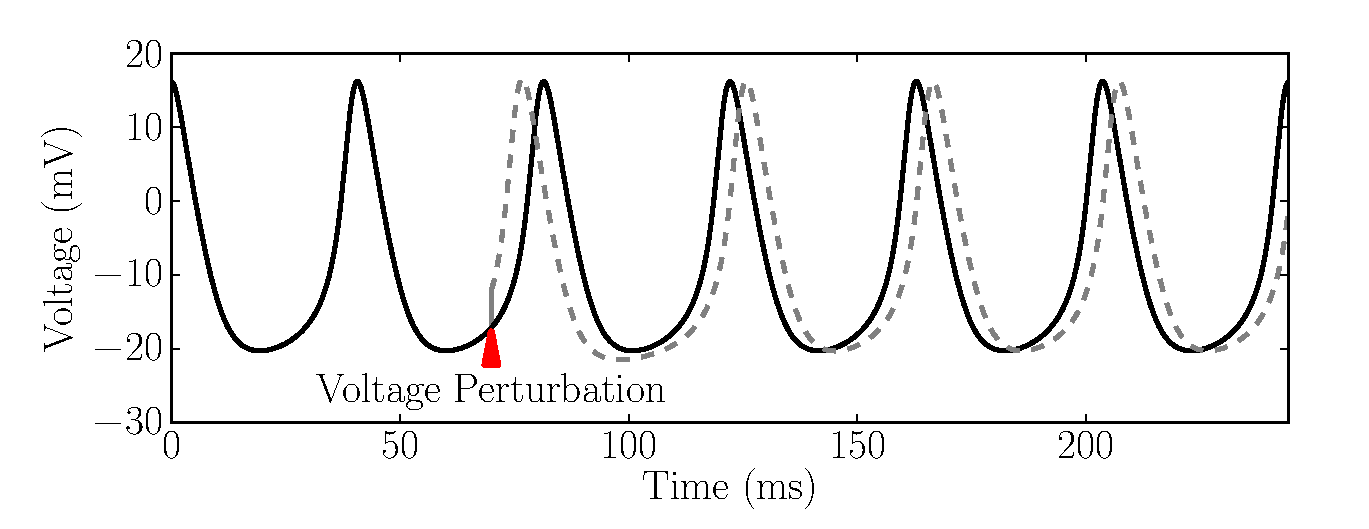
\includegraphics[width=1\textwidth]{voltage-pert-ml-vt.png}
%  \caption{Example of a phase response for the Morris-Lecar model: a voltage perturbation at phase $\phi \approx .6$ ($t \approx 70ms$) of a limit cycle leads to a change in timing of $\Delta \theta \approx .1$.  }
%  \label{fig:voltage-pert-ml}\end{figure}
%  
%       \begin{figure}[h!]
%  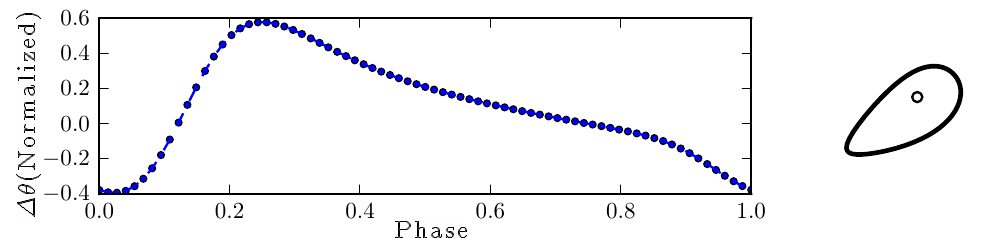
\includegraphics[width=1\textwidth]{voltage-pert-ml-quarter.png}
%  \caption{Example of an iPRC: Blue dots indicate the phase at which we apply an infinitesimal perturbation of size 1e-4 to the same model. The resulting phase difference is shown along the vertical axis.  The voltage over time plot from before is now shown in a phase space representation on the right.}
%  \label{fig:voltage-pert-ml-iprc}\end{figure}

\subsection{Infinitesimal Phase Response Curves and Differential Inclusions}\label{sec:iprcs_and_dis}
Differential inclusions are rigorously defined in \cite{Filipov1988}.  Here we consider a simplified definition. Let $B \subset \mathbb{R}^n$ be path connected.  A vector field $F:B \rightarrow \mathbb{R}^n$ is piecewise smooth on $B$ if there exist a finite number, $K$, of open sets $B_k$ such that
  \begin{enumerate}
    \item $B_k$ is nonempty, simply connected, and open for each $k$.
    \item $B_i \cap B_j = \varnothing, \forall i \neq j$.
    \item $B \subset \bigcup_{k=1}^K \bar{B}_k$.
    \item There exist smooth, bounded vector fields $F^k: \bar{B}_k \rightarrow \mathbb{R}^n$ such that for all $x$ in $B_k$, $F^k(x)=F(x)$.
  \end{enumerate}
  Note that we require $F^k=F$ only on the interior of each open domain $B_k$, while we require $F^k$ be smooth on the closure $\bar{B}_k$.  We also assume that the vector fields are arranged in such a way that a limit cycle exists.  In the basin of attraction of the limit cycle, we further assume that vector fields $F^k, F^{k+1}$ on adjacent sets $B_k,B_{k+1}$,  ``flow'' in the same direction at the boundary $\bar{B}_k \cap \bar{B}_{k+1}$ within a subset of the basin of attraction (Fig.~\ref{fig:general_regions}).  Finally, we assume that there exists a neighborhood about the point $\gamma^\partial$, within which the boundary is $C^1$.  Later we will specialize to the case where each vector field is defined by a system of linear equations.
   
   \begin{figure}[h!]
   \begin{center}
    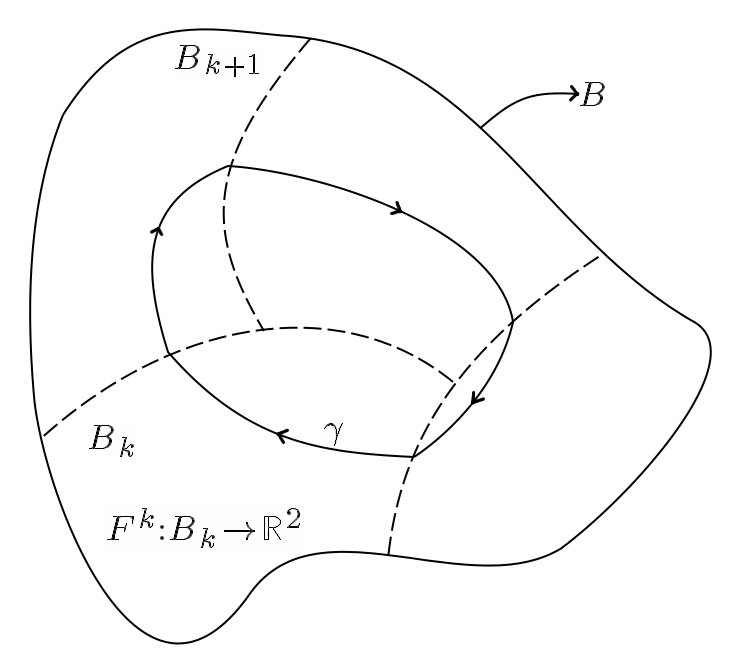
\includegraphics[width=.75\textwidth]{general_regions.png}
    \end{center}
    
    \caption[Example domains of a piecewise smooth dynamical system]{Example domains of a piecewise smooth dynamical system.  Each domain is separated by dashed lines.  A loop, $\gamma$, traversing all domains illustrates a limit cycle. See Figs.~\ref{fig:iris} and~\ref{fig:pml-appendix} for concrete examples of PWL models.}\label{fig:general_regions}
    \end{figure}

We now state several assumptions regarding limit cycles, phase, and isochrons.

\begin{enumerate}
 \item \textit{Existence and uniqueness holds for trajectories in the differential inclusions we consider.}
 
 Without giving a formal proof, we note that existence and uniqueness of trajectories holds within each domain $B_k$. By using the final coordinate of a trajectory $x^k$ in $B_k$ as the initial condition of a trajectory $x^{k+1}$ in $B_{k+1}$, we have the existence and uniqueness of the trajectory $x^{k+1}$ because the vector field defined over $B_{k+1}$ is smooth.  It seems plausible that existence and uniqueness for typical trajectories passing through multiple domains would follow by induction.
 
 \item \textit{The system has a stable limit cycle with well-defined phase.}
 
 Given existence and uniqueness of trajectories, there exist piecewise smooth vector fields with well-defined, isolated, $T$-periodic orbits. The phase of a $T$-periodic limit cycle in a piecewise smooth dynamical system follows naturally from the definition of phase, with $d\theta/dt = 1/T$.  By ``stable limit cycle'', we also mean to assume that the limit cycle is in the interior of an open set contained in the basin of attraction.
 
 \item \textit{A unique asymptotic phase exists for all points in the basin of attraction.}
 
 Existence and uniqueness of the asymptotic phase would follow from the assumed existence and uniqueness of solutions in the basin of attraction.
 
 \item \textit{Isochrons exist and are continuous.}
 
 Continuity of isochrons is equivalent to continuity of the phase function.  That is to say, for $x \in \Gamma$,
\begin{equation}
 \forall \varepsilon > 0, \exists \delta >0 \text{ s.t. } y \in B(x,\delta) \Rightarrow ||\theta(x)-\theta(y)|| < \varepsilon.
\end{equation}
We further assume that the asymptotic phase function satisfies
\begin{equation}
\frac{d\theta(x(t))}{dt} = 1/T, \quad \forall x(t) \in B.A.
\end{equation}
 
 \item \textit{$\theta(x)$ is locally differentiable at each domain boundary, in the direction tangent to the boundary.}
  Generally, the asymptotic phase function will not necessarily be differentiable in the direction transverse to the boundary.
\end{enumerate}

The definition of the iPRC does not apply directly to piecewise smooth differential equations.  For instance, the adjoint equation (Eqs.~\ref{eq:iprc_derivation} and ~\ref{eq:adjoint}) may not be solvable over a finite collection of sets, because the Jacobian may be ambiguous at the boundaries.  This problem of applying the adjoint equation to DIs has had limited attention.  Shaw et al. (2012) produced exact results for the iPRC of the iris system (a PWL model defined in Appendix \ref{app:iris}) using a direct derivation, but the method does not apply to general piecewise linear systems.  Coombes formulated a more general form for the iPRC of PWLDS and applied the theory to two planar PWL models \cite{Coombes:2008:SIADS}.  However, this method does not hold in cases where the iPRC is discontinuous, as it is for the iris system.  We now show how to solve for the iPRC for general planar piecewise smooth dynamical systems.

%\subsection{Thesis Outline}
%For the remainder of this thesis we focus on studying the infinitesimal phase response curve (iPRC) in two different contexts. In the first half, we explore the behavior of the iPRC with regards to general planar piecewise linear dynamical systems, and in particular, exactly how the iPRC behaves across boundaries between piecewise linear regions where the vector field may not be differentiable. We then apply this result to several piecewise linear systems.
\newpage
%
%To begin, I introduce the notion of phase response curves and the adjoint equation, which are the primary tools we use throughout the thesis.  I then detail the two main results, and conclude with a discussion.


%\section{The Adjoint Equation Across Boundaries of Piecewise Linear Planar Systems}

%\begin{itemize}
% \item (include a more precise title).  I'll organize the section as follows:
% \item Explain why the iris system may be used to approximate the sine system and why these results are useful.  it may be useful to use the adjoint equation from the iris system in the sine system.
% \item Not clear what is happening with the discontinuous jumps at boundary of regions
% \item solving the adjoint equation for a piecewise linear system and gaining insight into the jump of the iris iPRC at the boundary.
%\end{itemize}
\section[The iPRC of Piecewise Smooth Dynamical Systems]{The Infinitesimal Phase Response Curve of Piecewise Smooth Dynamical Systems}%.  A theorem quantifying discontinuities in the iPRC}
%In a previous result from Shaw \textit{et al}. (2012), we found discontinuous jumps in the iPRC of the iris system precisely at the boundaries between some piecewise linear regions.  
\subsection{Discontinuities of Infinitesimal Phase Response Curves of Differential Inclusions}
Consider a DI as constructed in Section \ref{sec:iprcs_and_dis}.  The vector field along the limit cycle may be discontinuous along domain boundaries, leading to discontinuity in the iPRC.  Our main result, Theorem \ref{theorem}, shows how to calculate these discontinuities. This expression, with the adjoint equation, constitute a complete picture of the iPRC of a DI.  %Since the theorem depends on having an exact expression for the iPRC, $z(t)$, we currently restrict ourselves to DIs with dynamics governed by linear differential equations.

\begin{figure}[h!]
\begin{center}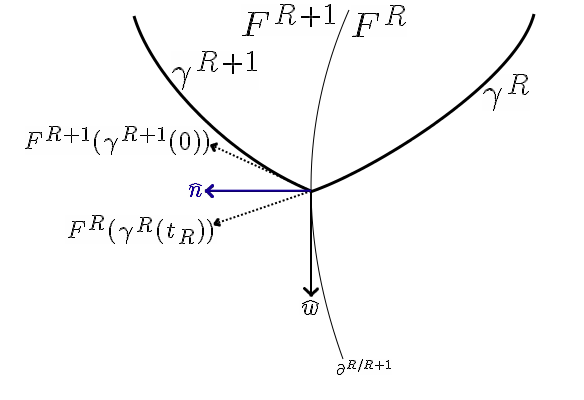
\includegraphics[width=.7\textwidth]{region_setup-revised.png}\end{center}
\caption[Piecewise smooth region setup and notation]{Piecewise smooth region setup and notation. The boundary separating the sets $B^R$ and $B^{R+1}$ (with vector fields $F^R$ and $F^{R+1}$, respectively) is denoted by $\partial^{R/R+1}$.  The limit cycle, $\gamma$, with solutions in region $R$ and $R+1$ (denoted $\gamma^R, \gamma^{R+1}$, respectively) is continuous across the boundary.  We use local time for $\gamma^R$ and $\gamma^{R+1}$ so that $\gamma^R(t_R) = \gamma^{R+1}(0)$, where $t_R$ is the time of flight through region $R$ (see Eq.~\eqref{eq:gamma_pieces}).  The values $F^R(\gamma(t_R)), F^{R+1}(\gamma(t_R))$ is the vector field in region $R,R+1$ at the point of egress and ingress, respectively, with vector $\hat{n}$ normal to the boundary and $\hat{w}$ tangent to the boundary.}
\label{fig:region_setup}
\end{figure}


 We first fix notation and define terms before introducing the theorem.   Let $F^R$ denote the vector field of region $R$, where each region is numbered according to the direction of flow within a neighborhood of the limit cycle, and assuming trajectories enter or exit transverse to the boundary with respect to each region.  The limit cycle, $\gamma$, is piecewise smooth, consisting of several curves $\gamma^1, \gamma^2, ... \gamma^K$. Each $\gamma^R$ spends a total time $t_R$ in its domain.  We write the limit cycle $\gamma$ as a collection of curves,
\begin{eqnarray}\label{eq:gamma_pieces}
  \gamma(t) = \left\{
  \begin{aligned}
    &\gamma^1(t), \quad 0=T_0 \leq t < T_1,\\
    &\gamma^2(t-T_1), \quad T_1 \leq t < T_2,\\
    &\vdots\\
    &\gamma^K \left ( t - T_{K-1} \right ), \quad T_{K-1} \leq t < T_K,
  \end{aligned}
  \right.
\end{eqnarray}
 where $T_i = \sum_{j=1}^i t_j$ and $\gamma^R(t_R) = \gamma^{R+1}(0)$.  The final and initial values of two adjacent vector fields, $F^R,F^{R+1}$, along the limit cycle are denoted
\begin{equation}\label{eq:vector-field-gamma}
F^{R+1}_0= \lim_{t \rightarrow 0^+} F^{R+1}(\gamma^{R+1}(t)),\hspace{1in} 
F^R_f= \lim_{t \rightarrow t_R^-} F^R(\gamma^{R}(t)).
\end{equation}
In Eq.~\eqref{eq:vector-field-gamma} and for the rest of the section, the value $t$ is taken to be local, i.e. the time elapsed since entering the current region.  The one-sided limits exist because each vector field is smooth on its domain.  The iPRC, $z(t)$, will be represented segment-by-segment with similar notation.  Define terms $z_f^R$ and $z_0^{R+1}$ by
\begin{align}
 z_f^R&=\lim_{t\to t_R^-}z^R(t),\\
 z_0^{R+1}&=\lim_{t\to 0^+}z^{R+1}(t),
\end{align}
where $z^R$ and $z^{R+1}$ are the solutions to the adjoint equation in regions $R$ and $R+1$, respectively.  Let $\psi_R$ be the angle of the vector normal to the boundary (with respect to a global Cartesian coordinate system) at which the limit cycle crosses the boundary.  Call this crossing point $\gamma^\partial$.  Finally, let $\hat{n} = (\cos\psi_R, \sin\psi_R)$ denote the unit vector normal to the boundary at $\gamma^\partial$, and let $\hat{w} = (-\sin\psi_R,\cos\psi_R)$ denote the unit vector tangent to the boundary at $\gamma^\partial$ (see Fig.~\ref{fig:region_setup}).  We now introduce the theorem.
\begin{theorem}
 Let $\gamma$ be a piecewise smooth limit cycle in $\mathbb{R}^2$ satisfying assumptions $1-5$ in Section \ref{sec:iprcs_and_dis}.  The iPRC for $\gamma$ satisfies the following boundary condition at the boundary $\partial^{R/R+1}$,
 \begin{equation}
z_0^{R+1}=M^R z_f^R,
\end{equation}
where
\begin{equation}
M^R = \matrix{cc}{f_0^{R+1} & g_0^{R+1}\\
-\sin\psi_R & \cos\psi_R}^{-1}\matrix{cc}{f_f^R & g_f^R\\
-\sin\psi_R & \cos\psi_R}.
\end{equation}
Existence of the required matrix inverse is guaranteed by the transverse flow condition, $F_0^{R+1}\cdot \hat{n} > 0$.
\label{theorem}\end{theorem}

\begin{proof}Recall that we assign asymptotic phase values $\theta(x)$ for points in the stable limit cycle $\Gamma$, and in its basin of attraction, B.A. The asymptotic phase function, $\theta$, is differentiable in the interior of each region and remains continuous at the boundaries.  The phase function is not necessarily differentiable on the boundaries with respect to space, but $\theta$ is always differentiable as a function of time, since we assume $d\theta(x(t))/dt = 1/T$ for any trajectory $x(t)$ in the basin of attraction.

These assumptions allow us to derive two linear equations satisfied by the iPRC, $z$, at each boundary.  Suppose we are at an arbitrary boundary between regions $R$ and $R+1$ (denoted $\partial^{R/R+1}$).  We denote the iPRC in regions $R$ and $R+1$ by $z^{R}, z^{R+1}$, respectively.  By the chain rule, for $k\in \{ R,R+1 \}$, we have the useful relation,
\begin{equation}
 \frac{d\theta}{dt}=F^{k}(x^{k}(t))\cdot\nabla\theta(x^{k}(t)).
\end{equation}
When $x^k(t) = \gamma^k(t)$, we have (by definition)
\begin{equation}
 \frac{d\theta}{dt} = F^{k}(\gamma^{k}(t))\cdot z^{k}(t).
\end{equation}
Recall that $d\theta/dt=1/T$. By taking the one-sided limits
\begin{equation}\label{eq:phase-limits}
 \begin{split}
  \lim_{t \rightarrow t_R^-} F^{R}(\gamma^{R}(t))\cdot z^R(t) &= F_f^{R}\cdot z_f^R,\\
  \lim_{t \rightarrow 0^+} F^{R+1}(\gamma^{R+1}(t))\cdot z^{R+1}(t) &= F_0^{R+1}\cdot z_0^{R+1},
  \end{split}
\end{equation}
we have the first equation relating $z^R$ and $z^{R+1}$,
\begin{equation}\label{eq:thetaflow}
F_f^{R}\cdot z_f^{R} = \frac{1}{T} = F_0^{R+1}\cdot z_0^{R+1}.
\end{equation}
Intuitively, Eq.~\eqref{eq:thetaflow} states that the phase function advances at the same rate as a function of time everywhere, and in particular on both sides of the boundary $\partial^{R/R+1}$, so the limits in Eq.~\ref{eq:phase-limits} must be equal.

To derive the second equation relating $z^R$ and $z^{R+1}$, we recall that the isochrons are continuous along each boundary, by assumption.  Define a coordinate, $w$, along the boundary such that the limit cycle crosses at $w=0$.  For some interval $w_{\text{min}}<0<w_{\text{max}}$, $w$ represents a point on the intersection of the boundary in B.A.  For any such point $w$, we can write the limit of the asymptotic phase function, $\theta^k$, from region $k \in \{ R,R+1 \}$, respectively, to the boundary as $\theta^k(w)$.  However, because isochrons are continuous across the boundary,
\begin{equation}
 \theta^R(w) = \theta^{R+1}(w).
\end{equation}


Moreover, by assumption, the partial derivatives of the isochrons with respect to $w$ coincide at the boundary, so
%Therefore, along the boundary there is an interval $w_{\text{min}}<0<w_{\text{max}}$ around the crossing point at $w=0$ such that for $w$ within this interval, the isochrons $\theta^I$ (extending continuously to the border from domain I) and $\theta^{R+1}$ (extending continuously to the border from domain R+1) coincide, i.e.~$\theta^R(w)=\theta^{R+1}(w)$.  By assumption, the partial derivatives of $\theta^{R/R+1}$ with respect to $w$ coincide at the boundary, so
\begin{equation}
\frac{d\theta^R}{dw}(w)=\frac{d\theta^{R+1}}{dw}(w),
\end{equation}
for any value of $w\in(w_{\text{min}},w_{\text{max}})$.  We can rewrite an equivalent expression using the directional derivative,
\begin{equation}
 \left(\nabla\theta^R(w)\right)\cdot\hat{w}=\left(\nabla\theta^{R+1}(w)\right)\cdot\hat{w}.
\end{equation}
In particular, for $w=0$, 
\begin{equation}
z^R(t_R)\cdot\hat{w}=z^{R+1}(0)\cdot\hat{w},
\end{equation}
which gives us our second equation,
\begin{equation}\label{eq:continuity}
z_f^R\cdot\hat{w} = z_0^{R+1}\cdot\hat{w}.
\end{equation}

We can combine equations (\ref{eq:thetaflow}) and (\ref{eq:continuity}) and rearrange as a system of equations,
%\begin{eqnarray}
%F^{R+1}_0\cdot z^{R+1}_0&=&F^R_f\cdot z^R_f,\\
%\hat{w}_R\cdot z^{R+1}_0&=&\hat{w}_R\cdot z_f^R.
%\end{eqnarray}
 \begin{eqnarray}
\matrix{cc}{f_0^{R+1} & g_0^{R+1}\\ -\sin\psi_R & \cos\psi_R}z_0^{R+1}
&=&
\matrix{cc}{f_f^R & g_f^R\\ -\sin\psi_R & \cos\psi_R}z_f^R.
\end{eqnarray}

The theorem follows upon left-multiplying the system by the inverse of the matrix on the left-hand side.  We are guaranteed invertibility as long as
\begin{equation}
 \det \matrix{cc}{f_0^{R+1} & g_0^{R+1}\\ -\sin\psi_R & \cos\psi_R} \neq 0.
\end{equation}
But by assumption, $\det \matrix{cc}{f_0^{R+1} & g_0^{R+1}\\ -\sin\psi_R & \cos\psi_R} = F_0^{R+1}\cdot \hat{n} > 0$. 
\qed
\end{proof}%$\Box$

We now focus on piecewise linear differential equations.


\begin{corollary}
With the assumptions of Theorem \ref{theorem} and affine linear vector fields $F^k$, the initial condition of the iPRC, $z(t)$, must satisfy
 \begin{equation}\label{eq:eigenvalue}
z^1_0=B z^1_0,
\end{equation}
where
\begin{equation}
B=M^{K}e^{A^{K}t_K}\cdots M^1e^{A^1 t_1},
\end{equation}
$t_k$ is the time of flight through the $k^{th}$ region, $e^{A^{k}}$ is the matrix exponential of $A^k = -\left(DF^k\right)^\intercal$.  Eq.~\eqref{eq:eigenvalue} and the normalization condition,
 \begin{equation}\label{eq:normalization}
F_0^1\cdot z^1_0=\frac{1}{T},
\end{equation}
yield a unique solution for the initial condition, $z_0^1 \in \mathbb{R}^2$, provided the nullspace of the matrix $B-I$ does not have dimension greater than one.
\label{corl:circuit}\end{corollary}

%It is straightforward to show that
%\begin{eqnarray}
%\det (M^R) &=& \frac{\hat{n}_R\cdot F^R_f}{\hat{n}_R\cdot F_0^{R+1}}\\
%\text{tr} (M^R)&=&1+\frac{\hat{n}_R\cdot F^R_f}{\hat{n}_R\cdot F_0^{R+1}}\\
%Q(M^R)=\text{tr}(M^R)^2-4\det(M^R) &=& \left( \frac{\hat{n}_R\cdot F^R_f}{\hat{n}_R\cdot F_0^{R+1}}-1 \right)^2
%\end{eqnarray}
%from which it follows that the eigenvalues of $M^R$ are exactly
%\begin{equation}
%\lambda\in\left\{1,\frac{\hat{n}_R\cdot F^R_f}{\hat{n}_R\cdot F_0^{R+1}}\right\}.
%\end{equation}
%Note that $\hat{n}_R\cdot F^R_f$ is the speed at which the limit cycle is traveling
%in the direction normal to the boundary when reaches crossing time $t_R$ from region $R$, and $\hat{n}_R\cdot F_0^{R+1}$ is the speed with which it enters region $R+1$, so the term showing up in the eigenvalues is the ratio of the normal velocity components  approaching and leaving the boundary.

%If, in addition, the flow is piecewise linear, with constant adjoint Jacobian matrices $A^R=-D(F^R)^\trans$, 
%and we define $\Delta_R=t_R-t_{R-1}$ to be the traversal time for region $R$, 
\begin{proof}
Let $z_0^1$ be the initial condition for the adjoint equation, and let $z_i^1(0)$ be the $i^{th}$ component.  To prove the corollary, we solve the adjoint equation for region $R$, apply the matrix $M^R$ at the boundary to calculate jumps in the iPRC, then repeat the process for region $R+1$ and continue inductively for subsequent regions.

Beginning with an arbitrary region, which we label $R=1$, the solution at $t_1$ (the time of flight through region $R=1$), is
\begin{equation}
 z^1_f = e^{A^1t_1}z^1_0,
\end{equation}
where $A(t) = -DF^T(\gamma(t))$ is constant.  The initial condition for the next region, $z_0^2$, is equal to the final value of the previous region with jumps calculated by $M^1$,
\begin{equation}
  z^2_0 = M^1 e^{A^1 t_1}z^1_0.
\end{equation}
We can continue this procedure inductively for the initial condition of the $K^{th}$ iPRC,
\begin{equation}
z^K_0=M^{K-1}e^{A^{K-1}t_{K-1}}\cdots M^1e^{A^1 t_1}z^1_0.
\end{equation}
Since the underlying limit cycle is periodic, $z(t)$ must be periodic, therefore $z^{K+1}(0) = z^1(0)$, and
\begin{equation}
 z^{1}_0=M^{K}e^{A^{K}t^{K}}M^{K-1}e^{A^{K-1}t^{K-1}}\cdots M^1e^{A^1t^1}z^1_0.
\end{equation}
The first statement in the corollary follows upon collapsing the matrix product into a $2\times2$ matrix $B$.

To prove uniqueness, we follow a procedure similar to that used in \cite{Coombes:2008:SIADS} and apply Eqs.~\eqref{eq:eigenvalue} and \eqref{eq:normalization}.  Rewriting Eq.~\eqref{eq:eigenvalue},
\begin{equation}
 \begin{split}
  \matrix{c}{z_1^1(0) \\ z_2^1(0)} &= z_0^1 =  B z_0^1\\
  &= \matrix{c}{b_{11} z_1^1(0) + b_{12}z_2^1(0)\\b_{21} z_1^1(0) + b_{22} z_2^1(0)}.
 \end{split}
\label{eq:Bmatrixfull}\end{equation}

we can rewrite Eq.~\eqref{eq:Bmatrixfull} as a system of equations for $z_1^1(0)$ and $z_2^1(0)$,
\begin{equation}
 \begin{split}
  z_1^1(0)(1-b_{11}) &= b_{12}z_2^1(0),\\
  z_2^1(0)(1-b_{22}) &=b_{21}z_1^1(0).
 \end{split}
\end{equation}

Without loss of generality, we choose the first of Eq.~\eqref{eq:Bmatrixfull} combined with Eq.~\eqref{eq:normalization} to form the system of equations,
\begin{equation}
 \begin{split}
 z_1^1(0) f_0^1 + z_2^1(0)g_0^1 &= \frac{1}{T},\\
  z_1^1(0)(b_{11}-1) + b_{12}z_2^1(0) &=0,
 \end{split}
\end{equation}
which we solve by inverting the matrix in the equivalent equation,
\begin{equation}
\matrix{cc}{f_0^1 & g_0^1\\(b_{11}-1) & b_{12}} \matrix{c}{z_1^1(0)\\z_2^1(0)} = \matrix{c}{\frac{1}{T}\\0},
\end{equation}
which establishes uniqueness of the solution, provided 
\begin{equation}\det \matrix{cc}{f_0^1 & g_0^1\\(b_{11}-1) & b_{12}} \neq 0.\label{eq:uniqueness-of-initial-cond}\end{equation} 
From the periodicity of the solution $z(t)$, we know that $B$ has at least one eigenvector with unit eigenvalue.  The condition (\ref{eq:uniqueness-of-initial-cond}) is equivalent to requiring that the matrix $B-I$ have a null space of not greater than one dimension.
\qed%$\Box$
\end{proof}
% which yields
% \begin{equation}
%  \matrix{c}{z_1^1(0)\\z_2^1(0)} = \matrix{cc}{1/f_0^1 & 0\\\frac{b_{21}}{f_0^1 (1-b_{22})} & 1/(1-b_{22})}  \matrix{c}{\frac{1}{T} - \frac{1-b_{11}}{b_{12}} g_0^1\\0},
% \end{equation}

\begin{corollary}\label{corl:c0-vector-fields}
 Under the assumptions of Corollary \ref{corl:circuit}, if adjacent vector fields evaluated along the limit cycle, $F_f^R$ and $F_0^{R+1}$, are continuous at the boundary $\partial^{R/R+1}$, then the matrix $M^R$ is the identity.
\end{corollary}

\begin{proof}
Recall the form of the matrix $M^R$ from Theorem \ref{theorem},
 \begin{equation}
    M^R = \matrix{cc}{f_0^{R+1} & g_0^{R+1}\\
-\sin\psi_R & \cos\psi_R}^{-1}\matrix{cc}{f_f^R & g_f^R\\
-\sin\psi_R & \cos\psi_R}.
 \label{eq:mr-corollary}\end{equation}
 If the vector fields on the limit cycle, $F_f^R, F_0^{R+1}$ are $C^0$ (they agree at the boundary), then
 \begin{equation}
  \begin{split}
   f_f^R &= f_0^{R+1},\\
   g_f^R &= g_0^{R+1},
  \end{split}
 \end{equation}
 and the matrix product in Eq.~\eqref{eq:mr-corollary} reduces to the identity matrix.
\end{proof}

%As a condition for this equation to be solvable, the matrix $B$ has to have at least one unit eigenvalue.  In addition, we have not yet used the normalization condition

%where $T=\sum_{k=1}^N \Delta_k$ is the total period, or the sum of the transit times through all $N$ regions.  
%These two conditions (\ref{eq:eigenvalue} and \ref{eq:normalization}) should (we hope?) lead to a unique solution for $z^1_0$, and hence $z(t)$.  
\subsection{Applications}
\subsubsection{Piecewise Linear Morris-Lecar}
The Morris-Lecar model is a conductance-based planar neurobiological model developed to understand oscillations in barnacle muscle fiber \cite{MorrisLecar:1981} (see Appendix \ref{app:morris-lecar}).  In \cite{Coombes:2008:SIADS}, Coombes constructed a piecewise linear approximation to the Morris-Lecar model for use in gap junction coupled networks (see Appendix \ref{app:pml}).  Coombes provides an ad-hoc derivation of the iPRC, implicitly taking the matrix $M^R$ to be the identity for each boundary crossing. Here we apply Corollary \ref{corl:c0-vector-fields} and show that $M^R$ is indeed the identity for all boundaries.

Let the piecewise linear Morris-Lecar be defined as in Appendix \ref{app:pml}.  The model contains three distinct vector fields, separated by vertical gray lines in Fig.~\ref{fig:pml-appendix}.  In the parameter regime we consider, the limit passes through the two rightmost boundaries, at $v = b = 0.5$ and $v = (1+a)/2 = 0.625$ (see Table \ref{table:param} for parameter values).

Along the boundary at $v = 0.5$, the first component, of the vector field, $\dot{v} = (f(v)-w+I)/C$, does not change over the boundary, so the first component agrees on both sides.  However, the second component of the vector field changes and each side is by definition,
 \begin{displaymath}
   g(v,w) = \left\{
     \begin{array}{lr}
       (v-\gamma_1w+b^*\gamma_1-b)/\gamma_1, \quad v < b\\
       (v-\gamma_2w+b^* \gamma_2-b)/\gamma_2, \quad v \geq b
     \end{array}
   \right.
\end{displaymath}
Let $g^4$ and $g^1$ denote the second component of the vector field to the left and right of the boundary.  Along the boundary, $v = b$, so the difference in the vector fields at the boundary is
\begin{equation}
\begin{split}
g^4(b,w) - g^1(b,w) &= (-\gamma_1w+b^*\gamma_1)/\gamma_1- (-\gamma_2w+b^* \gamma_2)/\gamma_2 \\
&= 0.
\end{split}
\end{equation}
Therefore, the vector field agrees on both sides at the boundary for all points along the boundary.  In particular, the vector field evaluated along any limit cycle is continuous at the boundary, so $M^R$ is the identity by Corollary \ref{corl:c0-vector-fields}.

We observe similar behavior at the boundary $v = 0.625$.  By definition, the second component of the vector field remains invariant when $v = 0.625$, while the first component of the vector field changes over this boundary,
\begin{equation}
 \begin{split}
  f(v) = \left \{ \begin{array}{ll} -v,& \quad v< a/2  \\
  v - a, & \quad a/2 \leq v \leq (1+a)/2 \\
  1- v, & \quad v >(1+a)/2 \end{array} \right .,
 \end{split}
\end{equation}
where $\dot{v} = (f(v) - w + I)/C$. We consider $f$ alone, since other parameters remain the same over the boundary.  Let $f^1$ and $f^2$ denote the first component to the left and right of the boundary.  The difference $f^1-f^2$ is
\begin{equation}
\begin{split}
 f^1\left((1+a)/2,w\right) - f^2\left ((1+a)/2,w\right ) &= (1+a)/2 - a - \left (1-(1+a)/2\right )\\
 &= 0.
\end{split}
\end{equation}
Again, the vector fields evaluated along any limit cycle agree at the boundary, so the matrix $M^R$ is the identity by Corollary \ref{corl:c0-vector-fields}.

Since the matrix $M^R$ is the identity for each boundary crossing of the limit cycle, the iPRC is continuous (though not necessarily $C^1$).  See Fig.~\ref{fig:pml_iprc} for the numerical iPRC that confirms this result.

\begin{figure}[h!]
\begin{center} 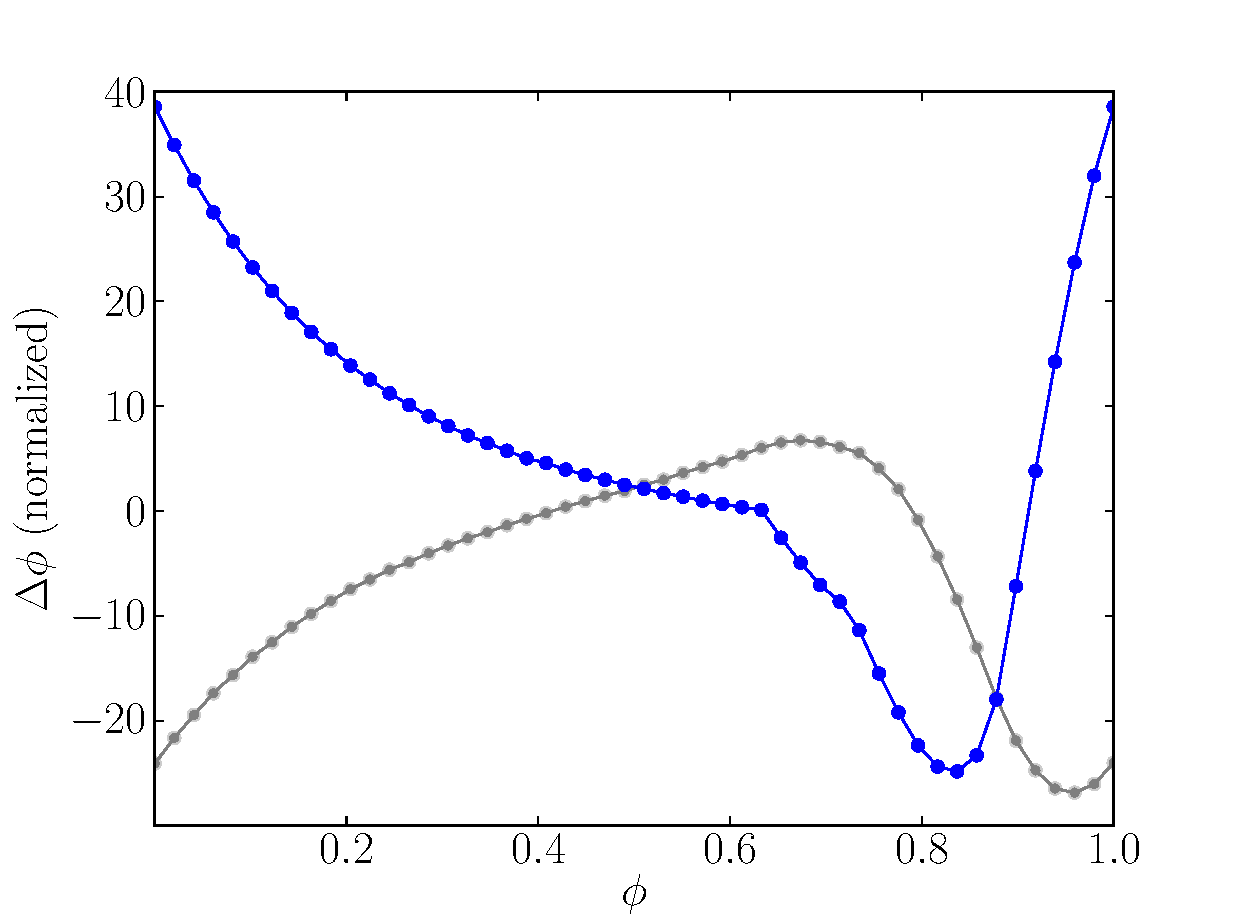
\includegraphics[width=1\textwidth]{pml_prc_fig.pdf}\end{center}
\caption[Numerical iPRCs of the PML system]{Numerical iPRCs of the PML system. Blue: perturbations in the positive horizontal direction. Gray: perturbations in the positive vertical direction.  There are no discontinuities in either iPRC \cite{Coombes:2008:SIADS}. Copyright~\copyright~~2008 Society for Industrial and Applied Mathematics.  Reprinted with permission.  All rights reserved.}
\label{fig:pml_iprc}\end{figure}

\subsubsection{McKean Model}
The McKean model is a piecewise linear approximation to the FitzHugh-Nagumo model \cite{McKean1970}.  Let the McKean model be defined as in Appendix \ref{app:mckean}.  We use similar methods as in the previous section. 

The limit cycle for the McKean model passes through both boundaries, at $v = a/2 = 0.125$ and $v = (1+a)/2 = 0.625$ (see Fig.~\ref{fig:mckean} and Table \ref{table:param} for parameter values).  The second component of the vector field is invariant over each boundary, so we consider just the function $f$ in the first component, $\dot{v} = (f(v) - w + I)/C$, since $f$ is the only term that changes at the boundaries.

At the leftmost boundary, $v = 0.125$, the difference in the function $f$ is,
\begin{equation}
\left . -v \right |_{v=a/2} - \left. (v-a) \right |_{v=a/2} = 0.
\end{equation}

At the rightmost boundary, $v = 0.625$, the difference in the function $f$ is,
\begin{equation}
\left . (v-a) \right |_{v=(1+a)/2} - \left. (1-v) \right |_{v=(1+a)/2} = 0.
\end{equation}
The vector field agrees on both sides at each boundary (and for vector fields evaluated along limit cycles in particular), so by Corollary \ref{corl:c0-vector-fields}, the matrix $M^R$ is the identity for each boundary crossing.

\begin{figure}[h!]
\begin{center} 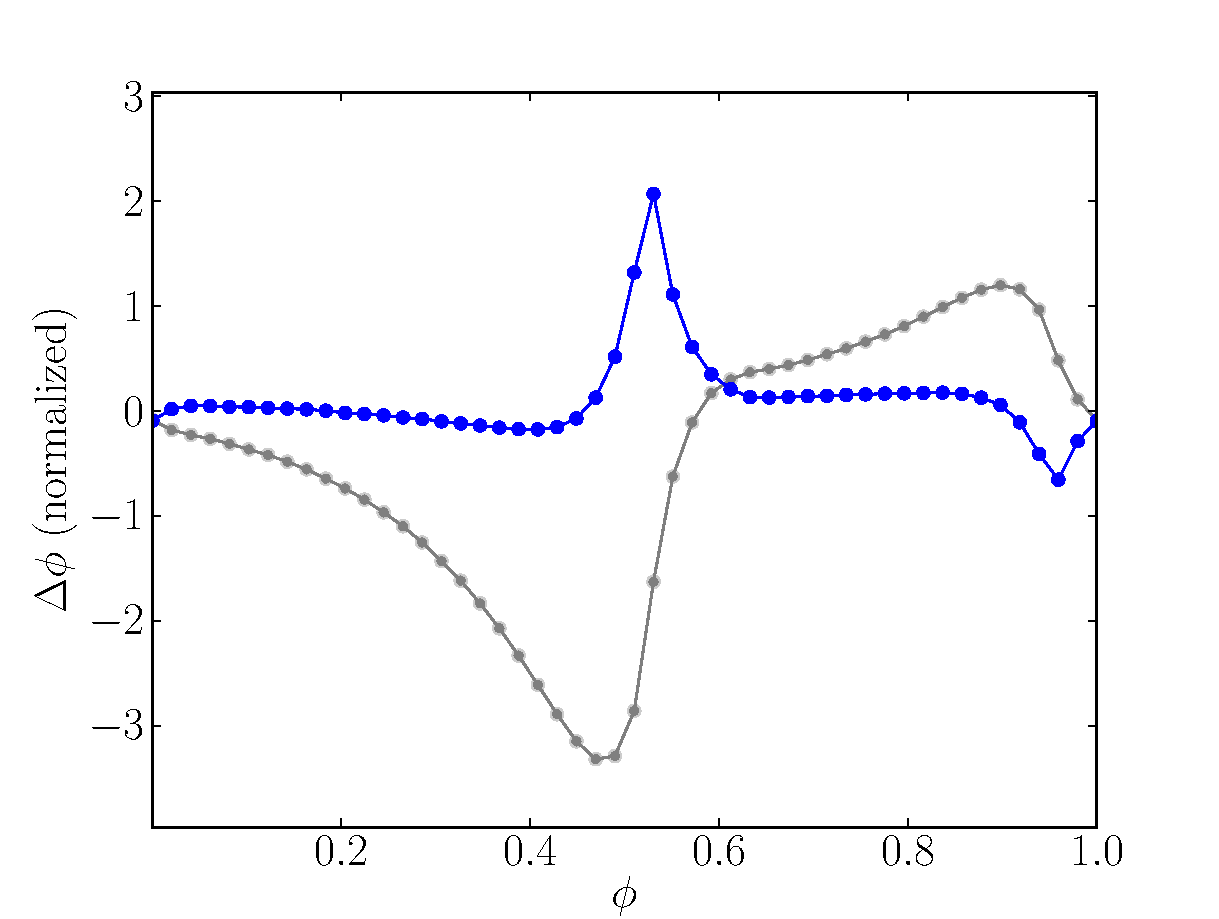
\includegraphics[width=1\textwidth]{pmk_prc_fig.pdf}\end{center}
\caption[Numerical iPRCs of the McKean model]{Numerical iPRCs of the McKean model. Blue: perturbations in the positive horizontal direction. Gray: perturbations in the positive vertical direction.  There are no discontinuities in either iPRC \cite{Coombes:2008:SIADS}. Copyright~\copyright ~2008 Society for Industrial and Applied Mathematics.  Reprinted with permission.  All rights reserved.}
\label{fig:pmk_iprc}\end{figure}

Again, the iPRCs of both coordinates are continuous (but not necessarily $C^1$).  See Fig.~\ref{fig:pmk_iprc} for the numerical iPRC that confirms this result.  We direct the reader to \cite{Coombes:2008:SIADS} for explicit expressions of the iPRC of the PML and McKean models.

\subsubsection{Iris System}
 The iris system is a piecewise linear dynamical system developed by Shaw et al. as an approximation to a particular smooth system, defined in Appendix \ref{app:sine}.  This smooth system, which Shaw et al. referred to as the sine system, was constructed to explore the effects of changing trajectories to pass closer to or further from saddle points by changing a single parameter. Both the sine system and iris system exhibit a family of limit cycles, indexed by a single parameter, which undergo a bifurcation to a heteroclinic cycle as the parameter goes to zero \cite{ShawParkChielThomas2012SIADS}.  Let the iris system be as defined in Appendix \ref{app:iris}.  When the corresponding bifurcation parameter, $a$, for the iris system, is small and positive, the iris system also produces a stable limit cycle (Fig.~\ref{fig:iris}). The limit cycle enters the Southwest region at coordinates $(1,u)$ and exits at coordinates $(s,1)= (u^\lambda,1)$, with transit time $T = \log(1/u)$, and enters the next region at local coordinates $(1,s+a)=(1,u)$.  Due to the symmetry of the iris system, the entry and exit coordinates of the other three regions are related by a 90-degree clockwise rotation, with each region having the same time of flight $T$. We define the phase $\theta = t/
T$ for each region.  As $a \rightarrow 0^+$, $u \rightarrow 0^+$, and the period $T$ diverges.

The dynamics in each square of the iris system is defined by a system of decoupled linear differential equations.  Therefore the Jacobian is a constant diagonal matrix, so the matrix exponential solution to the adjoint equation (Eq.~\ref{eq:adjoint}) is diagonal.  To solve for the initial conditions of the iPRC of the iris system, we use Corollary \ref{corl:circuit}.  First we obtain the matrix $B$ by solving the adjoint equation up to the time of flight beginning with the Southwest (SW) region, applying Theorem \ref{theorem} at the boundary between the SW and NW regions, then repeating inductively for the remaining three regions.  We solve for the initial conditions of the iPRC in the SW region using Corollary \ref{corl:circuit}.  The iPRC of the SW region is equivalent to the iPRC for the remaining regions up to rotation.

Let $(s,u)$ denote the local coordinates within an iris square, and $(x,y)$ denote the global coordinates of the iris system.  In each region the global coordinates differ from local coordinates by an affine rotation.  Consider the boundary between the SW and NW squares.  The dynamics in the SW square is
\begin{equation}
 F^{SW} = \matrix{c}{dx/dt \\ dy/dt} = \matrix{c}{-\lambda (x+c_{SW}) \\ y+d_{SW}} = \matrix{c}{-\lambda s\\ u},
\end{equation}
where the constants $c_{SW}$ and $d_{SW}$ offset the vector field.  The initial and final conditions of the vector field $F^{SW}$ evaluated along a limit cycle $\gamma$ with entry coordinates at $(1,u)$ and exit coordinates $(s,1)$, are
\begin{equation}
\begin{split}
 F_0^{SW} &= (-\lambda, u)^T,\\
 F_f^{SW} &= (-\lambda s, 1)^T.
\end{split}
\end{equation}
Its Jacobian is diagonal,
\begin{equation}
J_{SW} = \matrix{cc}{-\lambda & 0 \\ 0 & 1},
\end{equation}
and the solution to the adjoint equation, evaluated at the time of flight, is
\begin{equation}
z^{SW}(T) = \matrix{cc}{e^{\lambda T} & 0 \\ 0 & e^{-T}} z^{SW}(0).
\end{equation}
To obtain the jump condition matrix $M^R$ between SW and NW, we need to write the vector field of the next square, which is related to the SW square by 90-degree rotation,
\begin{equation}
 F^{NW} = \matrix{c}{dx/dt \\ dy/dt} = \matrix{c}{x+c_{NW} \\ -\lambda (y+d_{NW})} = \matrix{c}{u \\ -\lambda s},
\end{equation}
where $c_{NW}$ and $d_{NW}$ offset the vector field $F^{NW}$ and $s$ and $u$ are the (rotated) local coordinates.  The initial and final vectors of $F^{NW}$ along a limit cycle with the same entry and exit coordinates as before is related by the 90-degree rotation matrix, $\mathcal{R}=\matrix{cc}{0 & 1\\ -1 & 0}$.  Applying the rotation matrix to $F^{NW}$ returns the initial and final coordinates for $F^{NW}$ evaluated along the limit cycle,
\begin{equation}
\begin{split}
 F_0^{NW} &= \mathcal{R} F_0^{SW} = (u, \lambda)^T,\\
 F_f^{NW} &= \mathcal{R} F_f^{SW} = (1, \lambda s)^T.
\end{split}
\end{equation}
The Jacobian is
\begin{equation}
J_{NW} = \matrix{cc}{1 & 0 \\ 0 & -\lambda},
\end{equation}
and the solution to the adjoint evaluated at the time of flight is
\begin{equation}
z^{NW}(T) = \matrix{cc}{e^{-T} & 0 \\ 0 & e^{\lambda}} z^{NW}(0).
\end{equation}
By Theorem \ref{theorem},
\begin{equation}
\begin{split}
 M^{SW} &= \matrix{cc}{u & \lambda \\ -1 & 0}^{-1} \matrix{cc}{-\lambda s & 1 \\ -1 & 0}\\
 &= \matrix{cc}{-1 & 0 \\ s + \frac{u}{\lambda} & -\frac{1}{\lambda}}.
\end{split}
\end{equation}
%
So across the boundary,
\begin{equation}
\begin{split}
 z_0^{NW} &= \matrix{cc}{-1 & 0 \\ s + \frac{u}{\lambda} & -\frac{1}{\lambda}} z_f^{SW}.\\
 &= \matrix{cc}{-1 & 0 \\ s + \frac{u}{\lambda} & -\frac{1}{\lambda}} \matrix{cc}{e^{\lambda T} & 0 \\ 0 & e^{-T}}z_0^{SW},
\end{split}
\end{equation}
In the Northeast (NE) square, the dynamics are,
\begin{equation}
 F^{NE} = \matrix{c}{dx/dt \\ dy/dt} = \matrix{c}{- \lambda (x+c_{NE}) \\ (y+d_{NE})} = \matrix{c}{-\lambda s \\ u},
\end{equation}
where $c_{NE},d_{NE}$ are the constants offsetting the vector field in the NE square, and $s$ and $u$ are local coordinates within the NE square.  Note that in terms of the local coordinates, $F^{NE}$ and $F^{SW}$ have the same form, consistent with the rotational symmetry of the system.  The initial and final values of the vector field $F^{NE}$ evaluated along the limit cycle is related by a 90-degree rotation,
\begin{equation}
\begin{split}
 F_0^{NE} &= \mathcal{R} F_0^{NW} = (\lambda,-u)^T,\\
 F_f^{NE} &= \mathcal{R} F_f^{NW} = (\lambda s, -1)^T.
\end{split}
\end{equation}
The Jacobian is the same as in the SW square, so the solution to the adjoint is identical, with different initial conditions.  By Theorem \ref{theorem},
\begin{equation}
\begin{split}
 M^{NW} &= \matrix{cc}{\lambda & -u \\ 0 & 1}^{-1} \matrix{cc}{1 & \lambda s \\ 0 & 1}\\
 &= \matrix{cc}{\frac{1}{\lambda} & s + \frac{u}{\lambda} \\ 0 & 1}.
\end{split}
\end{equation}
The adjoint now consists of a product of four matrices,
\begin{equation}
\begin{split}
 z_0^{NE} &= \matrix{cc}{\frac{1}{\lambda} & s + \frac{u}{\lambda} \\ 0 & 1} \matrix{cc}{e^{\lambda T} & 0 \\ 0 & e^{-T}} z_0^{NW}\\
 %&=\matrix{cc}{\frac{1}{\lambda} & s + \frac{u}{\lambda} \\ 0 & 1} \matrix{cc}{e^{\lambda T} & 0 \\ 0 & e^{-T}} \matrix{cc}{-1 & 0 \\ s + \frac{u}{\lambda} & -\frac{1}{\lambda}} \matrix{cc}{e^{\lambda T} & 0 \\ 0 & e^{-T}} z_0^{SW}\\
 &= \matrix{cc}{\frac{e^{(\lambda-1)T}}{\lambda} - e^{2\lambda T} \left ( \frac{u}{\lambda} + s \right )^2, & \frac{e^{(\lambda-1)T}}{\lambda}\left ( \frac{u}{\lambda} + s \right )\\
 e^{2\lambda T} \left ( -\frac{u}{\lambda} -s \right), & \frac{e^{(\lambda -1)T}}{\lambda}}z_0^{SW}.
\end{split}
\end{equation}
The remaining jump matrices for the Northeast (NE) and Southeast (SE) squares, $M^{NE}$ and $M^{SE}$, are identical to the SW and NW squares, respectively.  Similarly, the Jacobian matrices of the NE and SE squares are the same as the corresponding matrices of the SW and NW squares.  Therefore the matrix $B$ of Corollary \ref{corl:circuit} is obtained by repeating the product of four matrices above,
\begin{equation}
\begin{split}
 z_0^{SW} &= B z_0^{SW}\\
 &= \matrix{cc}{\frac{e^{(\lambda-1)T}}{\lambda} - e^{2\lambda T} \left ( \frac{u}{\lambda} + s \right )^2, & \frac{e^{(\lambda-1)T}}{\lambda}\left ( \frac{u}{\lambda} + s \right )\\
 e^{2\lambda T} \left ( -\frac{u}{\lambda} -s \right), & \frac{e^{(\lambda -1)T}}{\lambda}}^2 z_0^{SW}.
\end{split}
\label{eq:iris-matrix-B}\end{equation}
Recalling that $e^{-T} = u$, and $e^{\lambda T} = 1/s$, it is straightforward to check that the matrix $B$ has an eigenvector $(s,1)^T$ with unit eigenvalue, so the initial condition of the iPRC is proportional to this vector, $z_0^{SW} \propto (s,1)^T$.  By Corollary \ref{corl:circuit}, the normalization condition $z_0^{SW} \cdot F_0^{SW} = 1/T$ determines the length of the vector $z_0^{SW}$.

Recalling that $s = u^\lambda$, in the SW square, $F_0^R = (-\lambda, u)^T$, so
\begin{equation}
\begin{split}
 z_0^{SW} \cdot F_0^{SW} &= s (-\lambda ) + u\\
 &=u - \lambda u^\lambda.
\end{split}
\end{equation}
Therefore, in order for $z_0^{SW} = (s,1) $ to satisfy the normalization condition, it must be scaled by the value $\frac{1}{T(u - \lambda u^\lambda)}$, which gives us our initial condition,
\begin{equation}
 z_0^{SW} = \left ( \frac{u^\lambda}{T(u - \lambda u^\lambda)}, \frac{1}{T(u - \lambda u^\lambda)} \right ).
\end{equation}
Combining this expression with the solution to the adjoint equation, $z(t)^{SW}$, and recalling that $t= \theta T = \theta \log(1/u)$, yields
\begin{equation}
\begin{split}
 z^R(t) &= \matrix{cc}{e^{\lambda t} & 0 \\ 0 & e^{-t}}z_0^R\\
 & = \matrix{cc}{e^{\lambda \theta T} & 0 \\ 0 & e^{-\theta T}} \matrix{c}{  \frac{u^\lambda}{T(u-\lambda u^\lambda)} \\ \frac{1}{T(u-\lambda u^\lambda)}  }\\
 & = \matrix{c}{  \frac{u^{\lambda(1-\theta)}}{T(u-\lambda u^\lambda)} \\ \frac{u^\theta}{T(u-\lambda u^\lambda)}  }.
\end{split}
\label{eq:new-derivation}\end{equation}

Expression \eqref{eq:new-derivation}is exactly the iPRC derived in \cite{ShawParkChielThomas2012SIADS}.  This alternative derivation is greatly simplified compared to the direct derivation in \cite{ShawParkChielThomas2012SIADS}, which involved the laborious task of keeping track of perturbed trajectories over an infinite series of boundary crossings.  In contrast, Theorem \ref{theorem} requires relatively simple calculations involving the vector fields, limit cycle, and adjoint equation, and extends naturally to general piecewise smooth dynamical systems.



\section{Discussion and Conclusions}
The infinitesimal phase response curve provides insight into how CPGs adaptively respond to perturbations including mechanical loads and sensory feedback.  Traditional CPG models are smooth, and the iPRC is obtained by numerically integrating the adjoint equation.  However, standard methods for obtaining the iPRC fail for flows with discontinuous vector fields.  We overcome this problem by deriving a boundary condition that allows integration of the adjoint equation around the limit cycle for such systems.  In the case of piecewise linear dynamics, this approach can lead to analytically exact expressions for the iPRC. Theorem \ref{theorem} provides a concise way to calculate an important portion of the iPRC for general planar DIs satisfying the assumptions in Section \ref{sec:iprcs_and_dis}, and improves upon two known methods for calculating the iPRC of DIs.

%The derivation from Shaw et al. (2012) for the iris system involves the direct, but laborious task of keeping track of infinitesimally perturbed trajectories along with information about their timing over an infinite sequence of boundary crossings.  The other derivation from Coombes (2008) uses more general methods that work well for FitzHugh-Nagumo-type models, including the McKean and PML models.  Central to Coombes's method is that the iPRC does not have any discontinuities at the boundaries, either by construction or assumption, so we can not apply the method to systems like the iris system, where the iPRC is discontinuous.  Theorem \ref{theorem} applies naturally to the Iris, McKean, and PML systems.

We did not cover a general method to solve the adjoint equation (Eq.~\ref{eq:adjoint}) within each piecewise linear domain because methods for solving coupled systems of linear differential equations are known.  In \cite{Coombes:2008:SIADS}, the coupled linear differential equations are solved by diagonalizing a matrix exponential, which provides an explicit form for the matrix $A$ in Eq.~\eqref{eq:adjoint}.  In the iris system, both state variables are decoupled, so solving for the adjoint is a matter of solving two separate linear differential equations and taking advantage of the special symmetry to derive a unique solution.  In \cite{ShawParkChielThomas2012SIADS} the iPRC was obtained through analysis of an infinite series capturing the compounded effects of offsets in position and time.  The method used by Shaw et al. would become intractable if applied to a system with different saddle values, $\lambda_i$, in each domain of the system.  For our method, by contrast, naturally includes systems in which the linear vector fields are not related by rotational symmetry, thereby providing a more flexible method for deriving the iPRC. For nonlinear dynamics, the adjoint equation may be solved numerically, by taking advantage of our jump condition.

Generalized iPRCs with periodic or random perturbations are beyond the scope of this discussion.  However, it is worth noting that if a limit cycle is strongly attracting, then the iPRC may be used to calculate the response of the system to either periodic or random perturbations.

%We have seen applications of Theorem \ref{theorem} to PWLDS, but the theorem extends naturally to piecewise smooth systems.  The exact expression of the iPRC  and the exact value of the discontinuity may not be known, but the theorem allows one to numerically calculate discontinuities at the boundaries.  This calculation, and the numerically computed solution to the adjoint in each region the approximate iPRC for differential inclusions.  

There are numerical advantages to our method as well.  The iPRC for a DI (and indeed for any system with a limit cycle) is traditionally derived by perturbing a limit cycle in phase space and tracking the asymptotic change in phase.  This direct simulation, while providing an accurate approximation to the iPRC, can be computationally expensive.  For example, one must evaluate a perturbed trajectory for several limit cycle periods to approximate the asymptotic phase, and one must repeat this calculation as many as one hundred times.  By using the theorem, the iPRC can be solved with as little as two limit cycle evaluations, one to find the period and limit cycle trajectory, and the other to solve the adjoint equation over each piecewise smooth region.

The main result of this thesis should prove useful in the continued use of piecewise smooth dynamical systems and phase response curves in mathematical biology.  Research in coupled oscillators has typically been restricted to smooth systems, or piecewise linear systems \cite{Coombes:2008:SIADS}.  Our result allows for the possibility for using a broader class of dynamical systems to study biological oscillators.  Finally, it is possible to derive exact expressions for the iPRC resulting from mechanical perturbations using piecewise linear dynamical systems.

In future work, we plan to extend the results of this thesis to $n$ dimensions.  The tools for smooth systems and many of our assumptions for piecewise smooth dynamical systems apply in $n$-dimensions.  Derivation of the matrix $M^R$ may include similar proof techniques.

\newpage
\appendix

%\section{Definitions}
\section{Appendix}
\subsection{Adjoint Equation}\label{app:adjoint_eq}
In this section we give an informal derivation of the adjoint equation satisfied by the infinitesimal phase response curve for a limit cycle in a smooth system of differential equations $dx/dt=F(x)$, introduced in Eq.~\eqref{eq:iprc_derivation}, namely:
\begin{equation}
 \frac{dz}{dt} = A(t) z(t),
\end{equation}
where $A(t) = -DF^T(x(t))$, and $z(t)=\nabla\theta(x(t))$.  For a more detailed proof, see \cite{BrownMoehlisHolmes:2004:NeComp}  or \cite{ErmentroutTerman2010book}.  Recall that
\begin{equation}
 \frac{d\theta}{dt} = \frac{1}{T}.
\end{equation}
Then
\begin{equation}\label{eq:adjoint-derivation}
\begin{split}
 0 &= \frac{d}{dt}\left(\frac{d\theta}{dt} \right)\\
 &=\frac{d}{dt}\left(\nabla\theta(x(t)) \cdot \frac{dx}{dt} \right)\\
 &=\left(\frac{d}{dt}\nabla\theta(x(t))\right) \cdot \frac{dx}{dt} + \nabla\theta\cdot\left(DF(x(t)) \frac{dx}{dt}\right)\\
 &=\left(\frac{d}{dt}\nabla\theta(x(t))\right) \cdot \frac{dx}{dt} + DF^T(x(t)) \nabla\theta \cdot \frac{dx}{dt}\\
 &=\left [ \frac{d}{dt} \nabla \theta(x(t)) + DF^T(x(t)) \nabla\theta(x(t)) \right ] \cdot F(x(t)).
\end{split}
\end{equation}

We assume that $F(x(t)) \neq 0$ and that the dot product in the last line of Eq.~\eqref{eq:adjoint-derivation} does not reduce to zero, so 
\begin{equation}
 \begin{split}
  \frac{d}{dt}& \nabla \theta(x(t)) + DF^T(x(t)) \nabla\theta(x(t)) = 0\\
  \Leftrightarrow \frac{d}{dt}& \nabla \theta(x(t)) = -DF^T(x(t)) \nabla\theta(x(t)).
 \end{split}
\end{equation}
When $x(t)$ is taken to be on the limit cycle, we recover the adjoint equation,
\begin{equation}
 \frac{dz}{dt} = -DF^T(\gamma(t)) z(t).
\end{equation}



\subsection{Model Equations}
In this section we provide, as a reference, the model equations for various systems discussed in the main text.  
\subsubsection{Morris-Lecar}\label{app:morris-lecar}
One well-studied neurobiological model capable of producing oscillatory behavior is the Morris-Lecar model.  The model was developed by Cathy Morris and Harold Lecar in 1981 to describe the many oscillations in barnacle muscle fiber \cite{MorrisLecar:1981}.  It is a conductance-based model with two state variables, so one may think of the model as a simplified model of Hodgkin-Huxley type.  The equations for the Morris-Lecar system are as follows:
\begin{equation}
{\begin{array}{rl}
C \frac{dV}{dt}&=I-g_L(V-E_L)-g_k n (V-E_K) - g_{Ca} m_\infty (V)(V-E_{Ca}), \\
\frac{dn}{dt}&=\phi (n_\infty(V) - n)/\tau_n(V),
\end{array}}
\end{equation}
where
\begin{equation}
 \begin{split}
m_\infty(V) &= \frac{1}{2} \left [ 1 + \tanh((V-V_1)/V_2) \right]\\
\tau_n(V) &= 1/\cosh((V-V_3)/(2V_4))\\
n_\infty(V) &= \frac{1}{2}\left [ 1 + \tanh((V-V_3)/V_4) \right ]
 \end{split}
\end{equation}
$V$ is the membrane potential, $C$ is the membrane capacitance, I is the applied current, and $g_L$, $g_{Ca}$, and $g_K$ are the peak conductances of leak, calcium, and potassium, respectively.  The variable $n$ represents the potassium recovery variable, with $m_{\infty}$ and $n_{\infty}$ representing the steady state equations for the calcium and potassium gating variables, respectively.  The voltage variables $E_L$, $E_{Ca}$, $E_K$ represent the respective Nernst potentials of each ion.  The remaining voltage variables, $V_1$ through $V_4$, determine the phase-plane properties of the model.  The variable $\phi$ depends heavily on temperature and affects the time constant, $\tau_n$, for the recovery variable, $n$, and in effect determines how quickly the membrane potential recovers.

%Though every parameter plays an important role in governing the types of oscillations exhibited by the model, the variables $I$ and $\phi$ stand out especially where $I$ stands for the amount of current applied to the barnacle muscle and $\phi$ determines how quickly the membrane potential recovers.

In phase space, $\phi$ controls the bifurcation regime and $I$ serves as a bifurcation parameter within each regime.  There are three main regimes of the ML system: Hopf, saddle-node on an invariant circle (SNIC), and homoclinic.  The regime is controlled by the parameter $\phi$, and bifurcations within each regime is controlled by $I_{app}$ (Table \ref{table:ml-param}).

\begin{table}[h!]
\centering
\caption{Parameter values for the Morris-Lecar model \cite{ErmentroutTerman2010book}.}
%of Fig.~\ref{fig:mckean} (Coombes 2008).}
    \begin{tabular}{  l | l | l | l }
    \hline
    Parameter	& Hopf	& SNIC	& Homoclinic \\ \hline
    $\phi$	& 0.04	& 0.067	& 0.23	 \\ \hline
    $g_{Ca}$	& 4.4	& 4	& 4	\\ \hline
    $V_3$	& 2	& 12 	& 12	\\ \hline
    $V_4$	& 30 	& 17.4	& 17.4	\\ \hline
    $E_{Ca}$ 	& 120	& 120 	& 120	\\ \hline
    $E_{K}$	& -84	& -84 	& -84	\\ \hline
    $E_L$	& -60 	& -60 	& -60 	\\ \hline
    $g_K$	& 8 	& 8 	& 8 	\\ \hline
    $g_L$	& 2 	& 2 	& 2 	\\ \hline
    $V_1$	& -1.2 	& -1.2 	& -1.2	\\ \hline
    $V_2$	& 18 	& 18 	& 18  	\\ \hline
    $C_m$	& 20 	& 20 	& 20	
    \end{tabular}
\label{table:ml-param}\end{table}


\subsubsection{McKean}\label{app:mckean}
The McKean model, first studied by Henry McKean \cite{McKean1970}, 
was introduced as a piecewise linear analog to planar conductance-based models such as the Morris-Lecar model. We use the parameters in Table \ref{table:mckean-param}.

The model equations are,
\begin{equation}
 \begin{split}
  C \dot{v} &= f(v) - w + I,\\
  \dot{w} &= g(v,w),
 \end{split}
\label{eq:coombes-eqs}\end{equation}
where the functions $f$ and $g$ are given by
\begin{equation}
 \begin{split}
  f(v) = \left \{ \begin{array}{ll} -v,& \quad v< a/2  \\ v - a, & \quad a/2 \leq v \leq (1+a)/2 \\ 1- v, & \quad v >(1+a)/2 \end{array} \right . ,
 \end{split}
\end{equation}
and
\begin{equation}
 g(v,w) = v - \gamma w.
\end{equation}
Figure \ref{fig:mckean} illustrates the $(v,w)$ phase plane for the McKean model.
%
\begin{figure}[h!]
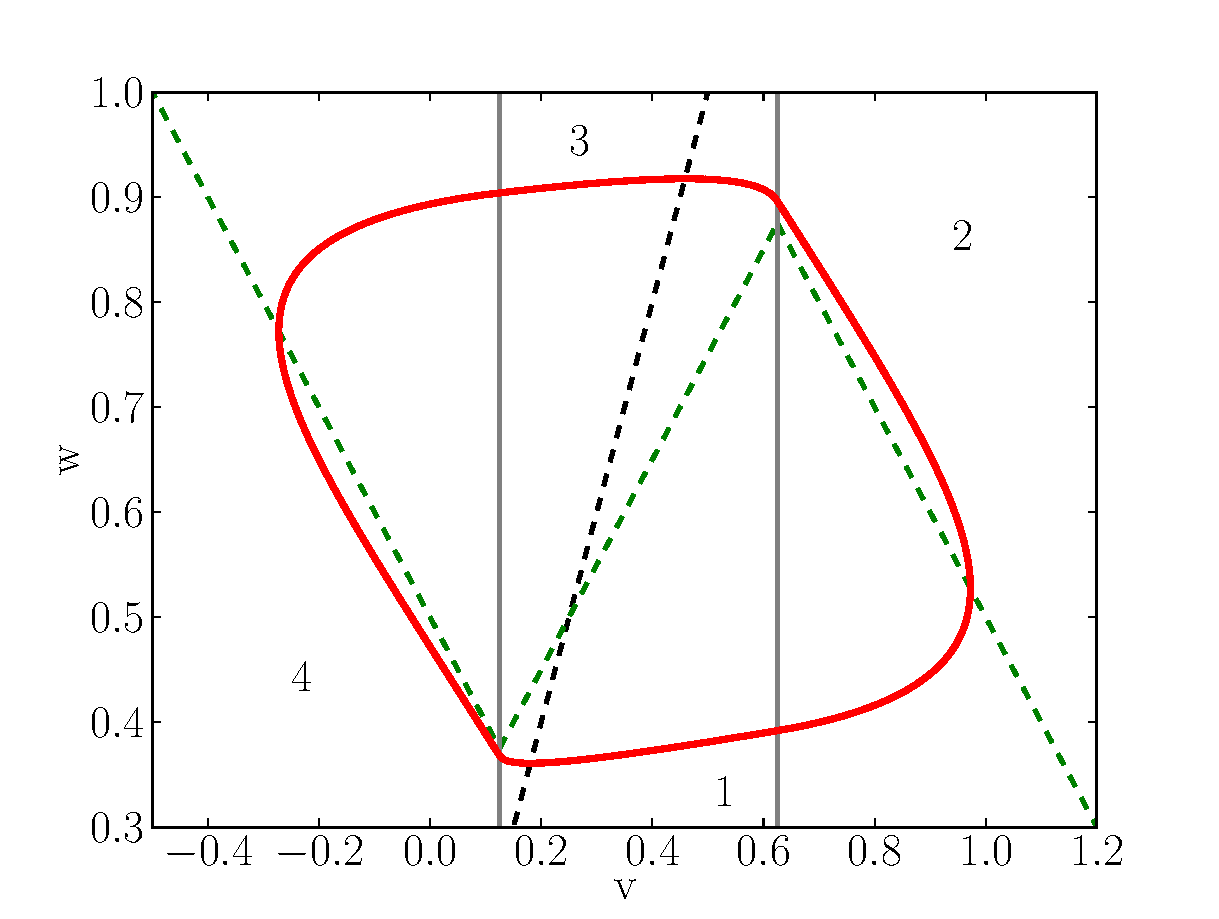
\includegraphics[width=\textwidth]{pmk_fig.pdf}
\caption[McKean model]{McKean model.  The black and green dashed lines represent the nullclines. The red loop represents the limit cycle.  Vertical gray lines denote the boundaries between each region (labeled 1 through 4) \cite{Coombes:2008:SIADS}. Copyright~\copyright~2008 Society for Industrial and Applied Mathematics.  Reprinted with permission.  All rights reserved.}
\label{fig:mckean}\end{figure}
%
\begin{table}[h!]
\centering
\caption{Parameter values for the McKean model \cite{Coombes:2008:SIADS}.}
%of Fig.~\ref{fig:mckean} (Coombes 2008).}
    \begin{tabular}{  l | l }
    \hline
    Parameter & Value \\ \hline
    $\gamma$ & .5 \\ \hline
    C & .1 \\ \hline
    a & 0.25 
    \end{tabular}
\label{table:mckean-param}\end{table}

\subsubsection{Piecewise Linear Morris-Lecar}\label{app:pml}
The Piecewise Linear Morris-Lecar system (PML system), studied in \cite{Coombes:2008:SIADS}, is a PWL approximation to the Morris-Lecar model.  We were motivated to study this model because of the relative simplicity of the equations and the availability of closed-form expressions for the iPRC and trajectories in phase space, from \cite{Coombes:2008:SIADS}.  The iris system, a PWL approximation of the sine system, provided insight into the behavior of the iPRC of the sine system.  We hoped to gain similar insight into the Morris-Lecar model by analyzing the PML model.

The equations for Coombes's PML model are the same as for the system in Eq.~\eqref{eq:coombes-eqs}, with parameters defined in Table 1.  The function $f(v)$ is defined as in the McKean model, and $g(v,w)$ is given by \cite{Coombes:2008:SIADS}:
 \begin{displaymath}
   g(v,w) = \left\{
     \begin{array}{lr}
       (v-\gamma_1w+b^*\gamma_1-b)/\gamma_1, \quad v < b\\
       (v-\gamma_2w+b^* \gamma_2-b)/\gamma_2, \quad v \geq b
     \end{array}
   \right.
\end{displaymath}
The nullclines are easily computed by hand and are illustrated in \ref{fig:pml-appendix}.

\begin{figure}[h!]
\begin{center}
 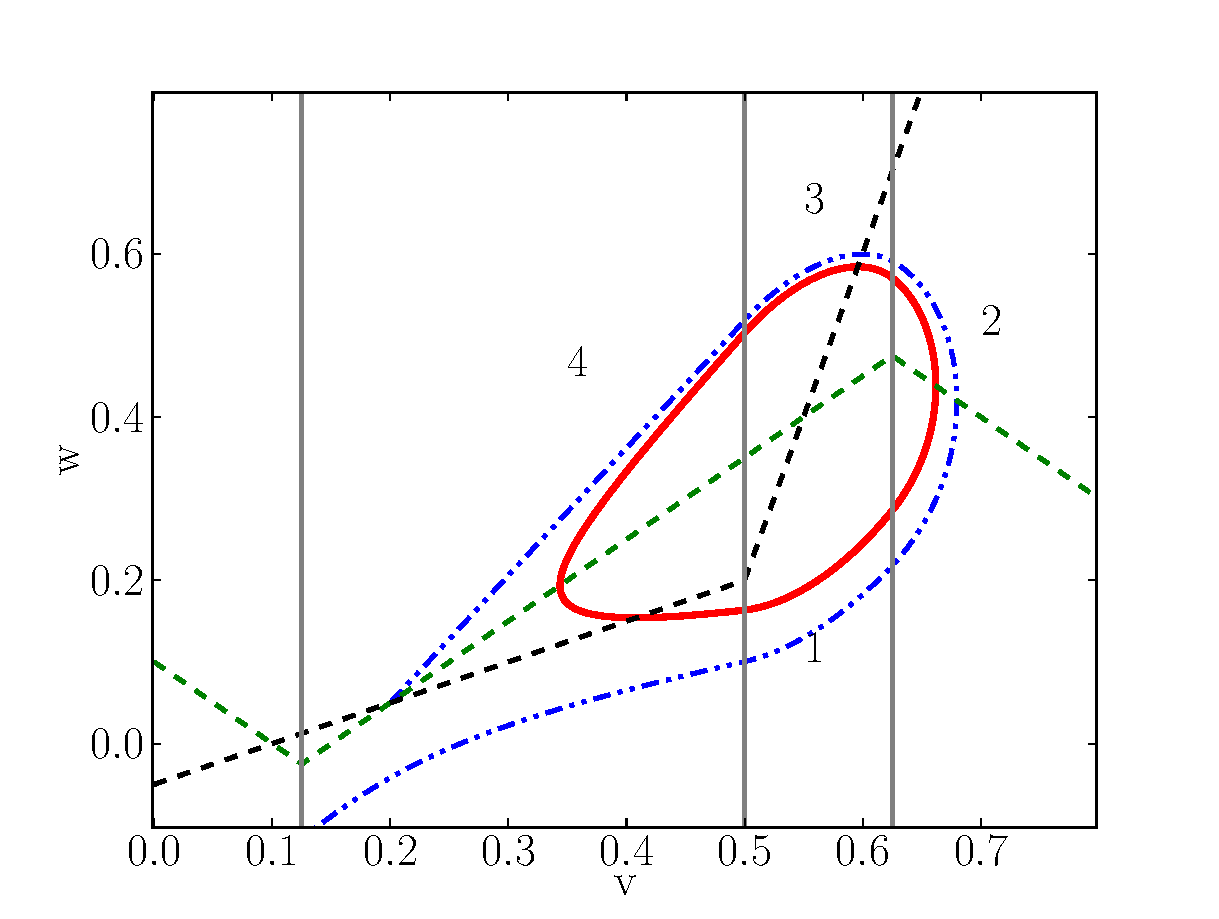
\includegraphics[width=1\textwidth]{pml_fig.pdf}
\end{center}
 \caption[Piecewise linear Morris-Lecar model]{Piecewise linear Morris-Lecar model.  The black and green dashed lines represent the nullclines.  The red loop represents the limit cycle, with the separatrix (represented by the blue dot-dot-dash), dividing the set of points that converge to the fixed point to the far left with points in the basin of attraction of the limit cycle.  Vertical gray lines denote the boundaries between each region (labeled 1 through 4).  The boundary between regions 4 and 1 is denoted $v_{th}^1$ and the boundary between regions 1 and 2 is denoted $v_{th}^2$ \cite{Coombes:2008:SIADS}. Copyright~\copyright~2008 Society for Industrial and Applied Mathematics.  Reprinted with permission.  All rights reserved.}
\label{fig:pml-appendix}\end{figure}


\begin{table}[h!]
\centering
\label{table:param}
\caption{Parameter values of the PML model (Fig.~\ref{fig:pml-appendix}) \cite{Coombes:2008:SIADS}.}
    \begin{tabular}{ l | l }
    \hline
    Parameter & Value \\ \hline
    $\gamma_1$ & 2 \\ \hline
    $\gamma_2$ & 0.25 \\ \hline
    C & 0.825 \\ \hline
    a & 0.25 \\ \hline
    b & 0.5 \\ \hline
    $b^*$ & 0.2

    \end{tabular}
\end{table}


\subsubsection{Sine System}\label{app:sine}
In \cite{ShawParkChielThomas2012SIADS}, Shaw et al. constructed the ``sine system'' as  a nominal model for systems with one-parameter families of limit cycles approaching close to a sequence of fixed points \cite{ShawParkChielThomas2012SIADS}. The sine system is a smooth planar system of autonomous ordinary differential equations defined as
\begin{equation}
 \begin{split}
  \frac{dy_1}{dt} &=f(y_1,y_2) = \cos(y_1)\sin(y_2) + \alpha \sin(2y_1),\\
  \frac{dy_2}{dt} &=g(y_1,y_2) = -\sin(y_1)\cos(y_2) + \alpha \sin(2y_2).
 \end{split}
\end{equation}
As written, the system forms a stable heteroclinic cycle, a special case of a heteroclinic channel \cite{AfraimovichTristanHuertaRabinovich:2008:Chaos}, where one unstable manifold of one saddle becomes the stable manifold of a neighboring saddle.  Limit cycles are introduced by breaking the heteroclinic cycle by perturbing the vector field by introducing an orthogonal component, whose magnitude is controlled by the parameter $\mu$.  These limit cycles have a close passage to each of the four saddle points in the system \cite{Reyn1980-bookchapter}.
\begin{equation}
 \begin{split}
  \frac{dy_1}{dt} &= f(y_1,y_2) + \mu g(y_1,y_2),\\
  \frac{dy_2}{dt} &= g(y_1,y_2) - \mu f(y_1,y_2),
 \end{split}
\end{equation}

where $1 > \mu > 0$. For any small $\mu >0$, there exists a stable limit cycle with diverging period as $\mu \rightarrow 0$.

\subsubsection{Iris System}\label{app:iris}
In order to derive analytical results, one may approximate the sine system with the iris system, a PWLDS \cite{ShawParkChielThomas2012SIADS}.  We use a linearization about one of the saddles in the sine system to construct four consecutive PWL regions, each a 90-degree rotation of the previous square.  For the sake of simplicity, we focus our analysis to the southwesterly (SW) iris square, and inject trajectories exiting the iris square (along the top edge) directly into the right edge of the same iris square, with a fixed offset $a\ge 0$.  Let $\lambda > 1$.  The nondimensionalized form of the iris equation is  
\begin{equation}
 \begin{split}
  \frac{ds}{dt} &= -\lambda s,\\
  \frac{du}{dt} &= u.
 \end{split}
\label{eq:iris}\end{equation}
Given initial condition $u(0)=u_0$ (and $s(0)\equiv 1$), if the first egress time is $T_1=\ln(1/u_0)$, with egress location $s(T_1^-)=u_0^\lambda$ (and $u(T_1^-)\equiv 1$), then after applying the offset the trajectory is reinjected at position $u_1=u(T_1^+)=s(T_1^-)+a=u_0^\lambda+a$.  Applying this procedure inductively, the successive injections occur at locations $u_{k+1}=u_k^\lambda+a$ and times $T_{k+1}=T_k+\ln(1/u_k)$.  

\begin{figure}[h!]
\begin{center}
 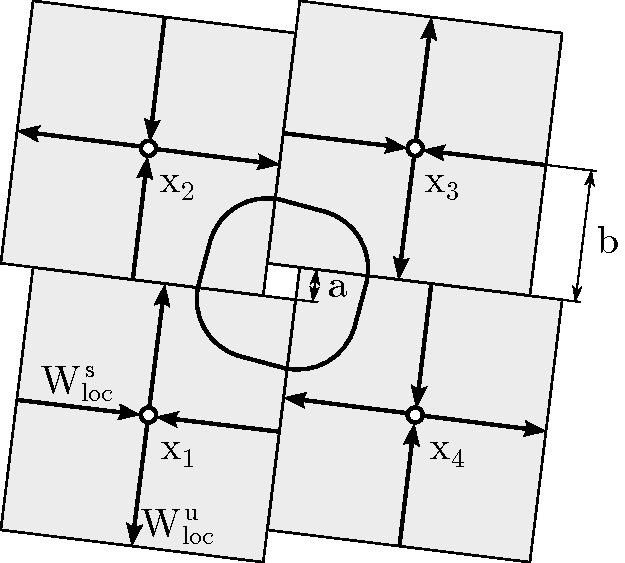
\includegraphics[width=.5\textwidth]{sine_to_iris_fig_sketch_iris.pdf}
\end{center}
\caption[Construction of the iris system]{Construction of the iris system.  The SW square is defined by the system in Eq.~\eqref{eq:iris}.  The remaining squares are defined by consecutive 90-degree clockwise rotation with a translation of system \eqref{eq:iris}.  The parameter $a$ acts as the bifurcation parameter (when $a=0$, there is a heteroclinic cycle), and the parameter $b = 1$. The unstable and stable manifolds of the saddle $x_1$ is denoted $W_{loc}^u$ and $W_{loc}^s$, respectively.  The loop passing through each  %piecewise 
region is an example of how a limit cycle might appear \cite{ShawParkChielThomas2012SIADS}. %look like. 
Copyright~\copyright~2012 Society for Industrial and Applied Mathematics.  Reprinted with permission.  All rights reserved.}\label{fig:iris}
\end{figure}


\subsection{Analytic, Piecewise Continuous Infinitesimal Phase Response Curve of the Iris System}\label{app:iris_summary}
\subsubsection{Summary of Shaw et al 2012}
In \cite{ShawParkChielThomas2012SIADS}, Shaw et al derived several analytical results for the iPRC of the iris system (see Appendix \ref{app:iris} for the definition).  The central result is a theorem which we summarize in three points.  Let $\lambda > 1 > a > 0$.
\begin{enumerate}
 \item If the function $\rho(u) = u^\lambda -u + a$ has two isolated positive roots, then the iris system has a stable limit cycle Moreover, the limit cycle trajectory enters each square at local coordinates $(1,u)$, where $u$ is one of the roots, and exits the square at local coordinates $(s,1)$, where $s = u^\lambda$.  The period of the limit cycle is $T = 4\log(1/u)$.
 \item The iPRC of the iris system, for perturbations in direction $\eta = (\eta_s,\eta_u)$ is
 \begin{equation}
  Z(\eta,\phi,a) = \frac{\eta \cdot \beta(\phi)}{\log(1/u)(u-\lambda s)},
 \end{equation}

 where $\phi = t/T$ is the phase, $\beta(\phi) = (s^{(1-\phi)}, u^\phi)$ and $\eta$ is a unit vector in the $L_1$ norm.
 \item The infinitesimal phase response to perturbations parallel to the unstable eigendirection in a given square diverges in the limit as $a \rightarrow 0$, and the response to perturbations parallel to the stable eigendirection diverges when $\phi \in (1-1/\lambda, 1)$; otherwise, the iPRC converges to zero as $a \rightarrow 0$.
\end{enumerate}
%
See Fig.~\ref{fig:iris-phase} for a geometric interpretation of this theorem.

\begin{figure}[h!]
\includegraphics[]{iris_prc_fig-revised.pdf}
 \caption[Divergence of the iris iPRC in the heteroclinic limit]{Divergence of the iris iPRC in the heteroclinic limit. As the theorem predicts, we have divergence of the iPRC of the iris system in the approach to the heteroclinic bifurcation.  The left column shows plots of the iPRC with phase change on the vertical axis and phase on the horizontal axis.  Dots represent values from numerical simulations and lines represent the analytic solution.  Bifurcation parameter values from top to bottom: $a=10^{-3},0.1,0.2$, and $0.24$ \cite{ShawParkChielThomas2012SIADS}.  Copyright~\copyright~2012 Society for Industrial and Applied Mathematics.  Reprinted with permission.  All rights reserved.}
\label{fig:iris-phase}\end{figure}

In order to gain a broader understanding of potential biological applications of these results and whether these results hold in general, we applied the same numerical tools to the Morris-Lecar system.  The Morris-Lecar system (defined in Appendix \ref{app:morris-lecar}) is a neurobiologically relevant dynamical system based on barnacle muscle.  The model is capable of several bifurcations, which include a hopf, saddle-node on a limit cycle (SNLC), and homoclinic bifurcation.  We focus on the homoclinic bifurcation because it provides an example of a family of limit cycles passing close to a single fixed point.  Once we are in a particular bifurcation regime, we generate limit cycles by varying a bifurcation parameter, $I_{app}$, which represents the current applied to the cell.

We used the python packages numpy and scipy to run perturbation analyses on the limit cycle of the Morris-Lecar model in the homoclinic regime.  Given a bifurcation parameter value $I_{app}$ (chosen such that a stable limit cycle exists) and a particular phase along the limit cycle, we use a perturbation of size $1\times 10^{-4}$ to estimate the change in timing at that phase.  By taking this analysis close to the homoclinic bifurcation, we find that the behavior of the iPRC in the approach to the homoclinic bifurcation closely resembles that of the analytic results of the iris system.  The peak sensitivity appears to diverge in the limit of the homoclinic bifurcation, while regions of relatively small sensitivity widen and dominate the behavior in the same homoclinic limit.

\begin{figure}[h!]
\includegraphics{morris-lecar_prcs-revised.pdf}
 \caption[Divergence of the Morris-Lecar iPRC in the homoclinic limit]{Divergence of the Morris-Lecar iPRC in the homoclinic limit.  The left column shows plots of the iPRC with phase change on the vertical axis and phase on the horizontal axis.  Zero phase, $\phi = 0$, defined to be peak voltage.  Perturbations of size $10^{-4}$ were used to construct the iPRC.  Bifurcation parameter values from bottom to top: $I_{app} = 40,36.2,35.05$, and $35.009$.  The bifurcation is near $I_{app} = 35.0067$.  The right column shows the corresponding limit cycle in phase space \cite{ShawParkChielThomas2012SIADS}. Copyright~\copyright~2012 Society for Industrial and Applied Mathematics.  Reprinted with permission.  All rights reserved.}
\label{fig:ml-iprc}\end{figure}

Since the Morris-Lecar equation is nonlinear, it is virtually impossible to derive analytical results for the iPRC near the homoclinic bifurcation.  However, the ever-lengthening regions of relatively small phase change suggest a different approach to understanding what happens to the shape of the iPRC in the limit of the homoclinic bifurcation.  The long, flat regions of the iPRC are a result of trajectories spending long times in a small neighborhood in phase space, so it is likely that trajectories spend long times in the neighborhood of the saddle.  If we can view the iPRC in terms of a variable that takes space into account instead of time, we may be able to more precisely calculate the shape of the iPRC in the limit of the homoclinic bifurcation.  Therefore, in future work, we hope to gain greater understanding of the limit behavior of the iPRC in this case, by analysis of the phase response curve as a function of arc length rather than of phase.  

  %We have developed some understanding of the iPRC of the iris system and its behavior in terms of phase in the limit of the homoclinic bifurcation.  We also have numerical evidence that the same qualitative behavior holds in the limit of a homoclinic bifurcation (Morris-Lecar) as well as in the limit of another heteroclinic bifurcation (Sine).  In particular, we observed that in the limit of the homoclinic (heteroclinic) bifurcation, the shape of the iPRC appeared increasingly flat for most phases, and grew thin peaks for some.

%\begin{figure}\label{fig:iprc-caricature}
%\caption{[Caricature of the numerical ML iPRC in the limit of the bifurcation]}
%\end{figure}
% 
% \subsubsection{The iPRC in Terms of Arc Length}
% 
% One way to view the iPRC in terms of space is to use the arc length of the limit cycle.  When viewed in this light, the regions representing a relative lack of sensitivity collapse to a small interval of arc length, and the more sensitive regions widen considerably, leading to a ``kink'' in the iPRC for perturbations close to the (a) saddle Fig.~\ref{fig:ml-iprc-arc-length}.  Understanding this kink may aid in understanding the shape of the iPRC for general homoclinic (and heteroclinic systems exhibiting particular symmetry).
% 
% \begin{figure}[h!]
% \begin{center}
% \includegraphics[width=.8\textwidth]{morris-lecar_prc-arc.pdf}
% \end{center}
% \caption[A kink near the homoclinic limit (Morris-Lecar)]{A kink near the homoclinic limit (Morris-Lecar).  For an input current value of $I_{app} = 35.0086$ close to the homoclinic bifurcation, a pronounced kink forms.  The gray, dashed line indicates zero phase change, indicating that at the kink, there is a rapid transition from convergent to divergent sensitivity.}
% \label{fig:ml-iprc-arc-length}\end{figure}
% 
% We see this same kink in both the sine and iris systems.
% 
% \begin{figure}[h!]
% \begin{center}
% 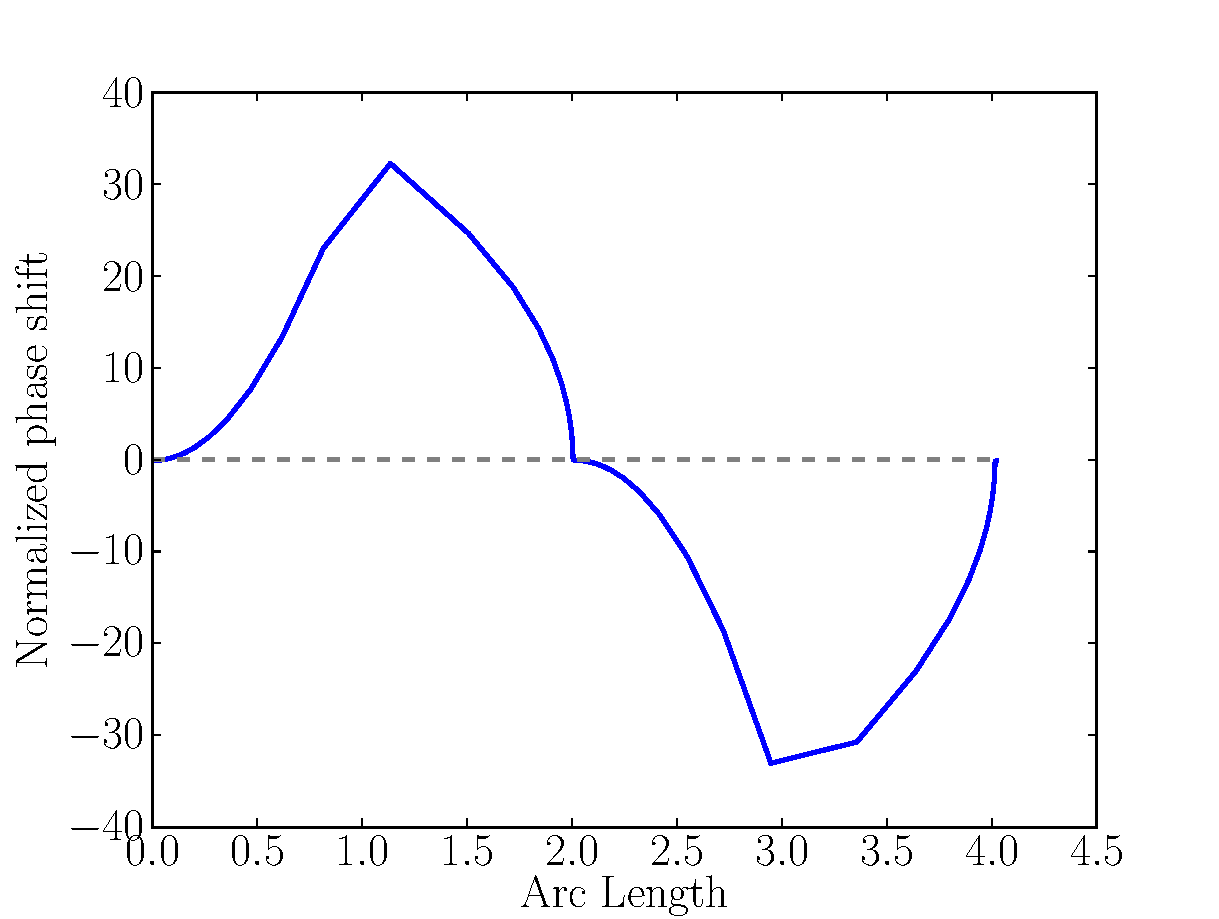
\includegraphics[width=.8\textwidth]{iris_prc-arc.pdf}
% \end{center}
% \caption[Two kinks near the heteroclinic limit (iris)]{Two kinks near the heteroclinic limit (iris).  One kink is located near zero arc length (arc length 4), and the other is located near arc length 2.  Both kinks are close to saddle points, just as in the Morris-Lecar model.  The kinks become sharper in the limit of the heteroclinic bifurcation.}
% \label{fig:iris-iprc-arc-length}\end{figure}
% 
% \begin{figure}[h!]
% \caption[Two kinks near the heteroclinic limit (sine)]{Two kinks near the heteroclinic limit (sine).  This sine system exhibits similar behavior.}
% \label{fig:sine-iprc-arc-length}\end{figure}
% 
% 
% 

\subsection{Normal Forms and Explicit Expressions for the Infinitesimal Phase Response Curve}\label{app:explicit_iprcs}
There are only a few cases where we can solve for the iPRC explicitly for smooth systems \cite{ErmentroutTerman2010book}.  Here we provide examples of explicit iPRCs which arise from normal forms for systems close to a particular bifurcation.  
\subsubsection{Class I Excitability}
Systems that always exhibit phase advance for perturbations along all phases are known as class I excitable systems.  Such systems typically make the transition from excitability to steady oscillation by way of a saddle-node-on-invariant circle (SNIC) bifurcation \cite{BrownMoehlisHolmes:2004:NeComp}.   The solution to the adjoint equation for the normal form a system at such a bifurcation is proportional to \cite{Ermentrout1996NeuralComput}
\begin{equation}
z(\theta) \propto 1-\cos(\theta).
\end{equation}

\subsubsection{Supercritical Hopf Bifurcation}
A model exhibits a supercritical Hopf bifurcation when the variation of a bifurcation parameter moves eigenvalues of a stable fixed point across the imaginary axis, leading to stable oscillations and an unstable fixed point.  The iPRC for models close to supercritical Hopf bifurcations may be approximated by a pure sinusoid \cite{BrownMoehlisHolmes:2004:NeComp,Izhikevich2007}.
\begin{equation}
z(\theta) \propto \sin(\theta).
\end{equation}


\newpage
\bibliographystyle{plain}
\addcontentsline{toc}{section}{References}
\bibliography{math,citations,Respiration,PJT,neuroscience}
%\bibliography{../../../papers/BibTex/neuroscience,../../../papers/BibTex/math,../../../papers/BibTex/PJT.bib,../../../papers/BibTex/misc.bib}


\end{document}